\chapter{Network Decompositions and DC Formulations}\label{ch:decompositions}

This chapter develops network decompositions that separate positive and negative contributions while preserving their difference. The DC instance exposes monotone, convex streams for the attribution methods of Chapter~\ref{ch:saliency}; the stopping instance preserves the gates underlying the games of Chapter~\ref{ch:game_theory}. Mixing and regularized decompositions connect these choices. Their shared forward invariant supports comparison of retained information and backward calculations; numerical stabilization makes them usable in deep networks.

\section{Generalized Network Decomposition}\label{sec:general_decomposition_def}

An ordinary signed activation combines opposing contributions into one number, hiding their magnitudes. Our decompositions replace it at every neuron and layer by a non-negative pair, exposing how supporting and opposing contributions accumulate while recovering the activation as their difference. Figure~\ref{fig:network_split_overview} illustrates the \ac{dc} instance of Section~\ref{sec:dc_splitting_relu}.

\begin{figure}[htbp]
	\centering
	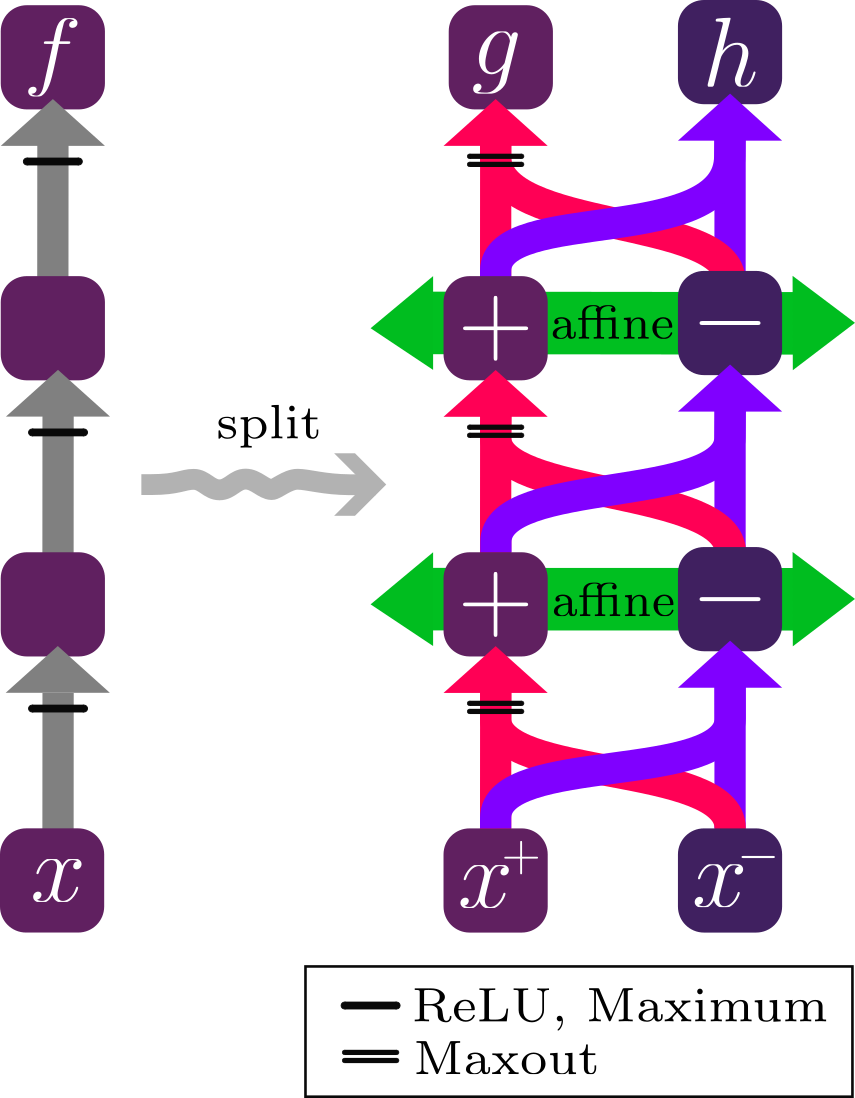
\includegraphics[width=0.28\textwidth]{figures/decompositions/network_split.png}
	\caption[The network splitting procedure]{The network splitting procedure: a \ac{relu} network $f$ is decomposed into two monotone, convex streams $g$ and $h$ with $f = g - h$ (Section~\ref{sec:dc_splitting_relu}).}
	\label{fig:network_split_overview}
\end{figure}

Consider an $L$-layer feedforward network with weights $\Wl{l}$, biases $b^{(l)}$, and entrywise activation $\varrho \colon \RR \to \RR$ (e.g.\ $\relu$ or softplus):
\begin{equation}
	\actl{0} = x,
	\qquad
	\preactl{l} = \Wl{l} \actl{l-1} + b^{(l)},
	\qquad
	\actl{l} = \varrho_l\bigl(\preactl{l}\bigr),
	\qquad l = 1, \dots, L,
	\label{eq:original_forward_pass}
\end{equation}
where $\varrho_l=\varrho$ for $1\leq l<L$ and $\varrho_L=\mathrm{id}$ gives the ungated affine readout $f(x)=\actl{L}\in\RR$. For multi-class networks, fix one target logit. We use the notation of Section~\ref{sec:nn_notation_pwl}, reserving $g,h$ for the split streams of Section~\ref{sec:dc_splitting_relu}.

A decomposition replaces each activation $\actl{l}_i$ by a non-negative pair propagated through non-negative linear maps and \emph{pairwise activation functions}. We first define this structure, then require its differences to recover the original network.

\begin{definition}[Decomposition]\label{def:decomposition}
A \emph{decomposition} of the $L$-layer network~\eqref{eq:original_forward_pass} propagates non-negative activation pairs $\bigl(\act{l}{+}_i, \act{l}{-}_i\bigr) \in \RR^2_{\ge 0}$ from input to output using only
\begin{enumerate}
	\item \textbf{non-negative linear maps}---matrices with non-negative entries together with non-negative bias vectors---and
	\item \textbf{pairwise activation functions} $\phi \colon \RR^2_{\ge 0} \to \RR^2_{\ge 0}$, $(z^+, z^-) \mapsto (a^+, a^-) = \phi(z^+, z^-)$, applied at every hidden neuron; the final affine readout uses the identity on the pair.
\end{enumerate}
Activations are indexed by $l \in \{0,\dots,L\}$, affine parameters by $l \in \{1,\dots,L\}$. The layer-$0$ pair is any non-negative split of the input,
\begin{equation}
	\bigl(\act{0}{+}_k, \act{0}{-}_k\bigr) \coloneqq \bigl(x_k^+, x_k^-\bigr),
	\qquad
	x_k^+ - x_k^- = x_k,
	\qquad
	x_k^+, x_k^- \ge 0,
	\label{eq:input_split_convention}
\end{equation}
and each affine layer $l$ maps the preceding activation pair to a non-negative pre-activation pair $\bigl(\preact{l}{+}_i, \preact{l}{-}_i\bigr)$. The pairwise activation applies for $l<L$; at $l=L$, $\act{L}{\pm}=\preact{L}{\pm}$. We call $\bigl(\act{l}{+}_i,\act{l}{-}_i\bigr)$ the \emph{decomposed activation} and $\bigl(\preact{l}{+}_i,\preact{l}{-}_i\bigr)$ the \emph{decomposed pre-activation}.
\end{definition}

\paragraph{Canonical non-negative linear map.}
We use the entrywise positive/negative split of the original weights and biases,
\begin{equation}
	\Wsig{l}{+} \coloneqq \posneg{\Wl{l}}{+},
	\qquad
	\Wsig{l}{-} \coloneqq \posneg{\Wl{l}}{-},
	\qquad
	b^{(l,+)} \coloneqq \posneg{b^{(l)}}{+},
	\qquad
	b^{(l,-)} \coloneqq \posneg{b^{(l)}}{-},
	\label{eq:canonical_weight_split}
\end{equation}
where $\posneg{\cdot}{\pm}$ are the entrywise positive and negative parts, so $\Wl{l} = \Wsig{l}{+} - \Wsig{l}{-}$ with $\Wsig{l}{\pm} \ge 0$. The resulting pre-activation pair at neuron $i$ is
\begin{align}
	\preact{l}{+}_i &\coloneqq b_i^{(l,+)} + \sum_j \Wsig{l}{+}_{ij}\, \act{l-1}{+}_j + \sum_j \Wsig{l}{-}_{ij}\, \act{l-1}{-}_j,
	\label{eq:split_pos}\\
	\preact{l}{-}_i &\coloneqq b_i^{(l,-)} + \sum_j \Wsig{l}{+}_{ij}\, \act{l-1}{-}_j + \sum_j \Wsig{l}{-}_{ij}\, \act{l-1}{+}_j.
	\label{eq:split_neg}
\end{align}
Positive weights preserve streams; negative weights swap them, turning excitatory contributions into inhibitory ones and vice versa. The following definition connects the structure of Definition~\ref{def:decomposition} to the original network.

\begin{definition}[Valid decomposition]\label{def:valid_decomposition}
A decomposition (Definition~\ref{def:decomposition}) is \emph{valid} for the network~\eqref{eq:original_forward_pass} with activation function $\varrho$ if the propagated activation pairs satisfy
\begin{equation}
	\act{l}{+}_i - \act{l}{-}_i = \varrho_l\bigl(\preactl{l}_i\bigr) = \actl{l}_i
	\label{eq:validity_condition}
\end{equation}
for every layer $l \in \{0, \dots, L\}$ and every neuron $i$, where at $l = 0$ condition~\eqref{eq:validity_condition} is read as $\act{0}{+}_k - \act{0}{-}_k = x_k$.
\end{definition}

Validity propagates through the canonical linear map, recovering the network output at the final layer.

\begin{proposition}[Validity recovers the network, \LeanResult{prop:validity_recovery}]\label{prop:validity_recovery}
Let a decomposition use the canonical non-negative linear map \eqref{eq:split_pos}--\eqref{eq:split_neg}. If the validity condition~\eqref{eq:validity_condition} holds at layer $l-1$, then the decomposed pre-activations at layer $l$ satisfy
\begin{equation}
	\preact{l}{+}_i - \preact{l}{-}_i = \preactl{l}_i
	\qquad \text{for every neuron } i.
	\label{eq:preactivation_difference}
\end{equation}
Consequently, every valid decomposition recovers the original network output as the difference of the final decomposed activations,
\begin{equation}
	f(x) = \act{L}{+} - \act{L}{-}.
	\label{eq:output_recovery}
\end{equation}\end{proposition}

\begin{proof}
Subtracting~\eqref{eq:split_neg} from~\eqref{eq:split_pos} and regrouping by predecessor $j$,
\begin{equation*}
	\preact{l}{+}_i - \preact{l}{-}_i
	= b_i^{(l,+)} - b_i^{(l,-)} + \sum_j \bigl( \Wsig{l}{+}_{ij} - \Wsig{l}{-}_{ij} \bigr) \bigl( \act{l-1}{+}_j - \act{l-1}{-}_j \bigr)
	= b_i^{(l)} + \sum_j \Wl{l}_{ij}\, \actl{l-1}_j
	= \preactl{l}_i,
\end{equation*}
The second equality uses $\Wl{l} = \Wsig{l}{+} - \Wsig{l}{-}$, $b^{(l)} = b^{(l,+)} - b^{(l,-)}$, and validity at layer $l-1$, proving~\eqref{eq:preactivation_difference}. At layer $L$, validity gives $\act{L}{+} - \act{L}{-} = \varrho_L\bigl(\preactl{L}\bigr) = \preactl{L} = f(x)$, proving~\eqref{eq:output_recovery}.
\end{proof}

By Proposition~\ref{prop:validity_recovery}, pre-activation differences recover the original pre-activations. A valid pairwise activation must therefore recover $\varrho(z^+-z^-)$ and preserve non-negativity on the input quadrant. Section~\ref{sec:dc_decompositions} gives conditions for convex, coordinatewise non-decreasing streams, constructs pairs from absolute curvature, and derives ReLU and smooth-activation formulas. Mixing (Section~\ref{sec:mixing_decomposition}), stopping (Section~\ref{sec:stopping_decomposition}), and regularized decompositions (Section~\ref{sec:regularized_decompositions}) preserve the same difference with other structural properties.

\section{Convex and Monotone DC Decompositions}\label{sec:dc_decompositions}

The required activation-level object is a pair of functions $F_+,F_-\colon\RR^2\to\RR$ satisfying
\begin{equation}
    \begin{gathered}
    \varrho(x-y)=F_+(x,y)-F_-(x,y),\\
    F_+,F_-\text{ convex and coordinatewise non-decreasing}.
    \end{gathered}
    \label{eq:general_dc_pair}
\end{equation}
Convexity alone is insufficient for recursive composition: a convex function of convex inputs need not be convex unless the outer function is non-decreasing in those inputs. Conversely, coordinatewise monotonicity does not mean that a function has non-negative values everywhere. We require the pair to be non-negative only on $\RR^2_{\ge0}$, the domain visited by the split network. The global domain $\RR^2$ in~\eqref{eq:general_dc_pair} makes the analytic requirements precise and permits signed inputs to the stream functions.

\subsection{The profile criterion and network composition}

Adding a common affine correction lifts a scalar DC decomposition $\varrho=p-q$ to such a pair. Here $L$ is a slope bound, independent of network depth. The criterion also covers ReLU's kink.

\begin{proposition}[Criterion for a convex, monotone pair, \LeanResult{prop:dc_profile_lift}]\label{prop:dc_profile_lift}
Let $L\ge0$ and $C\colon\RR\to\RR$, and define
\begin{equation}
    T_{C,L}(x,y)\coloneqq C(x-y)+Ly.
    \label{eq:dc_profile_lift}
\end{equation}
Then $T_{C,L}$ is convex on $\RR^2$ if and only if $C$ is convex. It is coordinatewise non-decreasing on $\RR^2$ if and only if
\begin{equation}
    0\le C(v)-C(u)\le L(v-u)\qquad(u\le v).
    \label{eq:dc_profile_increments}
\end{equation}
If $C$ is differentiable, condition~\eqref{eq:dc_profile_increments} is equivalent to $0\le C'\le L$. Consequently, given $p-q=\varrho$, the pair
\begin{equation}
    F_+(x,y)=p(x-y)+Ly,
    \qquad F_-(x,y)=q(x-y)+Ly
    \label{eq:asymmetric_dc_pair}
\end{equation}
is convex and coordinatewise non-decreasing exactly when both profiles are convex and satisfy~\eqref{eq:dc_profile_increments}. Under these conditions it maps $\RR^2_{\ge0}$ to itself exactly when $p(0),q(0)\ge0$.
\end{proposition}

\begin{proof}
Affine precomposition and affine addition preserve convexity; restriction to $y=0$ gives the converse. Increasing $x$ gives the lower bound in~\eqref{eq:dc_profile_increments}; increasing $y$ by $v-u$ changes the argument from $v$ to $u$, giving the upper bound. These inequalities also imply coordinatewise monotonicity. Difference quotients and the mean value theorem give the derivative criterion. The common $Ly$ cancels in $F_+-F_-$. On the non-negative quadrant, monotonicity gives $F_\pm(x,y)\ge F_\pm(0,0)$; evaluation at the origin proves necessity.
\end{proof}

\begin{theoremenv}[Network DC decomposition from activation pairs, \LeanResult{thm:general_dc_network}]\label{thm:general_dc_network}
Consider the network~\eqref{eq:original_forward_pass} with hidden activation $\varrho$. Choose a pair $F_+,F_-$ satisfying~\eqref{eq:general_dc_pair} on all of $\RR^2$ and $F_\pm(0,0)\ge0$. Use this pair entrywise after the canonical affine split~\eqref{eq:split_pos}--\eqref{eq:split_neg}, and use the identity pair at the final affine readout. Then every decomposed activation, and each of the two output streams $G,H$, is convex and coordinatewise non-decreasing as a function of the independent doubled input coordinates $(x^+,x^-)$. Moreover,
\begin{equation}
    G(x^+,x^-)-H(x^+,x^-)=f(x^+-x^-),
    \label{eq:general_network_dc_recovery}
\end{equation}
and both streams are non-negative when $x^+,x^-\ge0$. These conclusions also hold for every tail network starting at an intermediate layer.

If each component of an input split $x\mapsto(x^+(x),x^-(x))$ is convex, then $x\mapsto G(x^+(x),x^-(x))$ and $x\mapsto H(x^+(x),x^-(x))$ are convex. In particular, the usual split $x^\pm=\posneg{x}{\pm}$ gives a DC representation on the original input space.
\end{theoremenv}

\begin{proof}
The initial doubled coordinates are affine and non-decreasing. Non-negative affine combinations preserve convexity and coordinatewise monotonicity, as does composition with each convex, coordinatewise non-decreasing pair component. The final affine layer retains both properties. Induction proves the structural assertions for the network and every tail.

Subtracting each affine pair recovers the original affine map (Proposition~\ref{prop:validity_recovery}); each hidden pair gives $F_+(z^+,z^-)-F_-(z^+,z^-)=\varrho(z^+-z^-)$. The final identity pair gives the ungated pre-activation difference. Induction proves~\eqref{eq:general_network_dc_recovery}, including negative logits. Origin normalization and monotonicity preserve non-negativity at hidden layers, and canonical affine maps preserve it throughout. Composing a convex non-decreasing function with convex components proves the convex input-split assertion \parencite{Amos2017}.
\end{proof}

Monotonicity refers to independent pair coordinates. Under $x^\pm=\posneg{x}{\pm}$, convexity survives, while monotonicity in $x$ generally fails: $x^- =\max\{-x,0\}$ decreases with $x$. The theorem therefore gives monotone networks on doubled space and a DC representation on the original input space.

\subsection{Construction from absolute second derivatives}\label{sec:dc_splitting_smooth}

Finite positive and negative curvature gives bounded profile slopes. We construct them from $|f''|$, with $f$ now denoting a scalar activation.

\begin{theoremenv}[Absolute-curvature construction, \LeanResult{thm:absolute_curvature_split}]\label{thm:absolute_curvature_split}
Let $f\colon\RR\to\RR$ be differentiable, let $f'$ be locally absolutely continuous, and assume $f''\in L^1(\RR)$. Set
\begin{equation}
\begin{gathered}
    s_-\coloneqq\lim_{t\to-\infty}f'(t),\qquad
    V(t)\coloneqq\int_{-\infty}^{t}|f''(u)|\,\diff u,\\
    D(z)\coloneqq |f(0)|+|s_-|z+\int_0^z V(t)\,\diff t,\\
    p\coloneqq\frac{D+f}{2},\qquad q\coloneqq\frac{D-f}{2}.
\end{gathered}
    \label{eq:absolute_curvature_primitive}
\end{equation}
The limits $s_-$ and $s_+\coloneqq\lim_{t\to+\infty}f'(t)$ exist. With
\begin{equation}
    L\coloneqq\frac{\|f''\|_{L^1(\RR)}+|s_-|+|s_+|}{2},
    \label{eq:absolute_curvature_coefficient}
\end{equation}
the profiles $p,q$ are convex, satisfy $p-q=f$ and $0\le p',q'\le L$, and have $p(0)=\max\{f(0),0\}$, $q(0)=\max\{-f(0),0\}$. Therefore~\eqref{eq:asymmetric_dc_pair} is a convex, coordinatewise non-decreasing pair on $\RR^2$, is non-negative on $\RR^2_{\ge0}$, and recovers $f(x-y)$ exactly.
\end{theoremenv}

\begin{proof}
Local absolute continuity gives
$|f'(v)-f'(u)|\le\int_u^v|f''(t)|\,\diff t$ for $u\le v$.
Integrability makes $f'$ Cauchy at both ends of the real line, so its finite limits exist. Write
\begin{equation}
    P=\frac{|f''|+f''}{2},\qquad N=\frac{|f''|-f''}{2}.
    \label{eq:curvature_jordan_parts}
\end{equation}
Differentiating~\eqref{eq:absolute_curvature_primitive} yields
\begin{equation}
    p'(z)=\max\{s_-,0\}+\int_{-\infty}^z P(u)\,\diff u,
    \qquad
    q'(z)=\max\{-s_-,0\}+\int_{-\infty}^z N(u)\,\diff u.
    \label{eq:canonical_profile_slopes}
\end{equation}
Both derivatives are non-negative, non-decreasing, and bounded, and $p''=P$, $q''=N$ almost everywhere. Their upper limits are
$A=\max\{s_-,0\}+\int_{\RR}P$ and
$B=\max\{-s_-,0\}+\int_{\RR}N$.
Since $A+B=|s_-|+\|f''\|_1$ and $A-B=s_+$, their maximum is precisely~\eqref{eq:absolute_curvature_coefficient}. The difference and origin values follow directly from the definition. Proposition~\ref{prop:dc_profile_lift} now proves all pair properties.
\end{proof}

The functions $P$ and $N$ are the positive and negative parts of curvature. They are minimal: any twice weakly differentiable convex profiles $\widetilde p,\widetilde q$ with $\widetilde p-\widetilde q=f$ satisfy $\widetilde p''\ge P$ and $\widetilde q''\ge N$ almost everywhere. Within the affine lift~\eqref{eq:asymmetric_dc_pair}, the coefficient in~\eqref{eq:absolute_curvature_coefficient} is also the least possible common slope bound for globally convex non-decreasing profiles. Indeed, their non-negative limiting slopes at $-\infty$ differ by $s_-$, so they are at least $\max\{s_-,0\}$ and $\max\{-s_-,0\}$; their curvature measures dominate $P\,\diff z$ and $N\,\diff z$. Both upper slope bounds are therefore at least $A$ and $B$ from the proof. This is a minimality statement for this profile-and-affine-lift construction, not for arbitrary bivariate decompositions or for the sizes of the resulting network streams.

\begin{remark}[Why the global domain matters]\label{rem:global_curvature_necessity}
Under the regularity assumptions on $f'$ above, integrability of $f''$ is also necessary for the existence of \emph{finite-valued} convex, coordinatewise non-decreasing $F_+,F_-$ on all of $\RR^2$ with difference $f(x-y)$. To see this, restrict each component to $(t,0)$ for $t\le0$. The resulting convex non-decreasing function has slopes bounded between $0$ and a finite one-sided slope at the origin, hence finite curvature mass on the negative half-line. Next restrict each component to $(0,-t)$ for $t\ge0$. These restrictions are convex and non-increasing, so their slopes lie between a finite slope at the origin and $0$, giving finite curvature mass on the positive half-line. In both restrictions the difference is $f(t)$; the total variation of its curvature is bounded by the sum of the two positive curvature measures. Thus $\int_{\RR}|f''|<\infty$. This necessity argument concerns the global domain and does not apply if the pair is defined only on the non-negative quadrant. For example,
\begin{equation*}
    (x-y)^2=\bigl(2x^2+2y^2\bigr)-(x+y)^2
\end{equation*}
is a difference of two convex, coordinatewise non-decreasing functions on that quadrant, although the curvature of $f(z)=z^2$ is not integrable on $\RR$.
\end{remark}

\begin{corollary}[Exact splitting on a bounded activation interval]\label{cor:local_curvature_split}
Let $a<b$ and let $f\in C^1([a,b])$ have absolutely continuous derivative. There exist finite-valued convex, coordinatewise non-decreasing functions $F_+,F_-\colon\RR^2\to\RR$, non-negative on $\RR^2_{\ge0}$, such that $F_+(x,y)-F_-(x,y)=f(x-y)$ whenever $x-y\in[a,b]$.
\end{corollary}

\begin{proof}
Extend $f$ by its tangent affine functions at $a$ and $b$. The extension is continuously differentiable, its derivative is locally absolutely continuous, and its curvature vanishes outside $[a,b]$. Apply Theorem~\ref{thm:absolute_curvature_split} to this extension.
\end{proof}

This local statement applies, for example, to exponentiation on a fixed bounded score interval. It does not assert a global monotone convex split for $e^z$ on all of $\RR$, whose curvature is not integrable.

\subsection{ReLU: the maximum and identity pair}\label{sec:dc_splitting_relu}

For $f(z)=\relu(z)$ choose $p(z)=\relu(z)$, $q(z)=0$, and $L=1$. Both profiles are convex and satisfy~\eqref{eq:dc_profile_increments}, even though $p$ is not differentiable at the origin. The profile lift gives the exact pair
\begin{equation}
    \begin{gathered}
    F_+(a,b)=\relu(a-b)+b=\max\{a,b\},\qquad F_-(a,b)=b,\\
    \relu(a-b)=\max\{a,b\}-b.
    \end{gathered}
    \label{eq:splitting_identity}
\end{equation}
This specializes the general criterion to a positive Maxout component \parencite{Goodfellow2013Maxout} and a negative identity component. Replacing $f''\,\diff z$ by $\delta_0$ in the absolute-curvature construction gives the same pair (Remark~\ref{rem:bv_extension}). This classical ReLU-network DC split \parencite{Zhang2018,Siahkamari2020_DCRegression,Awasthi2023DCNN,hiddenMono} underlies our stabilized passes, CNN extension, and saliency methods.

The hidden-layer update is therefore
\begin{equation}
    \act{l}{+}=\max\{\preact{l}{+},\preact{l}{-}\},
    \qquad \act{l}{-}=\preact{l}{-},\qquad 1\le l<L,
    \label{eq:dc_split_activations}
\end{equation}
with $\act{L}{\pm}=\preact{L}{\pm}$ at the final affine readout. Theorem~\ref{thm:general_dc_network} gives validity and convexity. Section~\ref{sec:mixing_decomposition} identifies this as the mixing family's $\eta=1$ endpoint.

\begin{figure}[htbp]
	\centering
	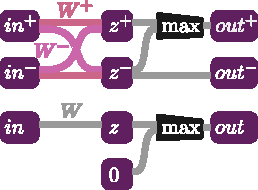
\includegraphics[width=.35\linewidth]{figures/decompositions/split_streams.pdf}
	\caption[Monotone, convex split streams and a standard ReLU layer]{Monotone, convex split streams (top) and a standard \ac{relu} layer (bottom). Negative weights swap positive and negative input streams into opposite pre-activation streams; positive weights preserve them.}
	\label{fig:splitstreams}
\end{figure}

\paragraph{The stream functions $g$ and $h$.}
The \ac{dc} \emph{split pair} consists of two monotone \emph{split streams}, non-negative on the input quadrant (Figure~\ref{fig:splitstreams}). Like the tail network $f^{(l)} \colon \RR^{d^{(l)}} \to \RR$ on layers $l+1, \dots, L$, define the restricted streams
\begin{equation}
	g^{(l)} \colon \RR^{d^{(l)}} \times \RR^{d^{(l)}} \to \RR,
	\qquad
	h^{(l)} \colon \RR^{d^{(l)}} \times \RR^{d^{(l)}} \to \RR,
	\label{eq:stream_functions}
\end{equation}
mapping an activation pair at layer $l$ to the $+$ and $-$ components of the decomposed output; we abbreviate $g \coloneqq g^{(0)}$, $h \coloneqq h^{(0)}$. On the output layer $g^{(L)}(x^+, x^-) = x^+$, $h^{(L)}(x^+, x^-) = x^-$, and for $0 \le l < L$,
\begin{equation}
	g^{(l)}(x^+, x^-) = g^{(l+1)}\bigl(\act{l+1}{+}, \act{l+1}{-}\bigr),
	\qquad
	h^{(l)}(x^+, x^-) = h^{(l+1)}\bigl(\act{l+1}{+}, \act{l+1}{-}\bigr),
	\label{eq:stream_recursion}
\end{equation}
where \eqref{eq:split_pos}--\eqref{eq:split_neg} and \eqref{eq:dc_split_activations} compute $\bigl(\act{l+1}{+}, \act{l+1}{-}\bigr)$ from $(x^+,x^-)$. These full tail functions, rather than individual layer activations, define $f=g-h$ and underpin Chapter~\ref{ch:saliency}. The \ac{mlp} split pass starts from $\bigl(\act{0}{+},\act{0}{-}\bigr)=(x^+,x^-)$, then applies the affine pair \eqref{eq:split_pos}--\eqref{eq:split_neg} and the maximum/identity update~\eqref{eq:dc_split_activations} for $l=1,\dots,L-1$. The final layer uses only the affine pair, allowing negative reconstructed logits.

Non-negative affine maps followed by Maxout gates and projections form monotone networks with convex, monotone activations. The composition principles of Section~\ref{sec:convex_monotone_foundations} \parencite{Amos2017} give:

\begin{proposition}[Monotonicity and convexity of the split streams, \LeanResult{prop:stream_properties}]\label{prop:stream_properties}
For every $0 \le l \le L$, the stream functions $g^{(l)}$ and $h^{(l)}$ of~\eqref{eq:stream_functions} are convex and non-decreasing in each coordinate of the pair $(x^+, x^-) \in \RR^{d^{(l)}} \times \RR^{d^{(l)}}$.\end{proposition}

\begin{proof}
Apply Theorem~\ref{thm:general_dc_network} to each tail network using the pair $(\max\{a,b\},b)$ from~\eqref{eq:splitting_identity}. The final pair is the identity, so the same argument includes the ungated affine head.
\end{proof}

The correctness statement asserts that the difference of the two split-stream outputs equals the original tail network evaluated at the difference of their inputs---at \emph{every} layer, not only at the input.

\begin{theoremenv}[Correctness of the split forward pass, \LeanResult{thm:split_correct}]\label{thm:split_correct}
For every $0 \le l \le L$ and all $x^+, x^- \in \RR^{d^{(l)}}_{\ge 0}$,
\begin{equation}
	f^{(l)}\bigl( x^+ - x^- \bigr)
	= \bigl( g^{(l)} - h^{(l)} \bigr)(x^+, x^-).
	\label{eq:split_correctness}
\end{equation}\end{theoremenv}

\begin{proof}
Apply Theorem~\ref{thm:general_dc_network} to each tail. Hidden-pair subtraction gives $\relu(z^+-z^-)$ by~\eqref{eq:splitting_identity}, and final-pair subtraction gives $z^+-z^-$ since $\varrho_L=\mathrm{id}$. The identity tail at $l=L$ and recursion~\eqref{eq:stream_recursion} give~\eqref{eq:split_correctness} at every layer.
\end{proof}

\begin{remark}[Preservation of sub-threshold signals]\label{rem:subthreshold}
At an inactive neuron, $\preactl{l}_i\le0$, ReLU outputs $\actl{l}_i=0$, discarding the losing pre-activation's magnitude. Downstream computation cannot distinguish degrees of suppression. The split pair $\bigl(\act{l}{+}_i,\act{l}{-}_i\bigr)=\bigl(\preact{l}{-}_i,\preact{l}{-}_i\bigr)$ has the required zero difference while retaining the cancelled mass $\preact{l}{-}_i$ in both components. These sub-threshold contributions give the streams more information than the original activations, which Chapter~\ref{ch:saliency} exploits. Retaining them also causes the numerical growth of Section~\ref{sec:stabilization_dc}: without subtractive cancellation, the streams accumulate absolute mass $\preact{l}{+}_i+\preact{l}{-}_i$ instead of the signed residual.
\end{remark}

\begin{remark}[Flexibility of the input split]\label{rem:input_split_flexibility}
Theorem~\ref{thm:split_correct} allows \emph{any} non-negative representation $x=x^+-x^-$, including $x^\pm=\posneg{x}{\pm}$ and $x^\pm=\posneg{x}{\pm}+c$ with $c\ge0$. Numerical stabilization and Chapter~\ref{ch:saliency}'s attribution baselines exploit this freedom. The half--half split $x^\pm=\pm x/2$ (Section~\ref{sec:stabilization_dc}) instead has signed components: it serves only as a backward chain-rule device along the unified input direction.
\end{remark}

\subsection{Closed formulas for smooth activations}\label{sec:closed_form_dc_activations}

The following activations admit explicit absolute-curvature profiles. Smooth curvature majorants yield shorter formulas, so we give both and distinguish exact recovery from minimal curvature. Write $\sigma(z)=(1+e^{-z})^{-1}$, let $\varphi,\Phi$ be the standard Gaussian density and distribution function, and set
\begin{equation*}
    s_\beta(z)\coloneqq\frac{1}{\beta}\log(1+e^{\beta z}),\qquad \beta>0.
\end{equation*}

\begin{corollary}[Explicit convex, monotone activation pairs, \LeanResult{cor:closed_form_dc_activations}]\label{cor:closed_form_dc_activations}
For $f(z)=z\Phi(z)$ (GELU), $f(z)=z\sigma(\beta z)$ (Swish), $f=\sigma$ (sigmoid), and $f=s_{1/\theta}$ (softplus), choose the corresponding row of Table~\ref{tab:closed_form_dc_profiles}. Then the functions $F_+(x,y)=p(x-y)+Ly$ and $F_-(x,y)=q(x-y)+Ly$ are convex and coordinatewise non-decreasing on $\RR^2$, map $\RR^2_{\ge0}$ to itself, and satisfy $F_+-F_-=f(x-y)$.
\end{corollary}

\begin{table}[htbp]
\TableContent{
\centering
\small
\setlength{\tabcolsep}{5pt}
\begin{tabularx}{\linewidth}{@{}l>{\raggedright\arraybackslash}X>{\raggedright\arraybackslash}Xc@{}}
\toprule
Activation & $p(z)$ & $q(z)$ & $L$ \\
\midrule
GELU & $2z\Phi(z)+2\varphi(z)$ & $z\Phi(z)+2\varphi(z)$ & $2$ \\[3pt]
Swish & $2s_\beta(z)$ & $2s_\beta(z)-z\sigma(\beta z)$ & $2$ \\[3pt]
Sigmoid & $\tfrac12(s_1(z)+\sigma(z))$ & $\tfrac12(s_1(z)-\sigma(z))$ & $\tfrac12$ \\[3pt]
Softplus & $s_{1/\theta}(z)$ & $0$ & $1$ \\
\bottomrule
\end{tabularx}
}%
\caption[Closed scalar profiles for smooth activations]{Closed profiles for~\eqref{eq:asymmetric_dc_pair}, $\beta,\theta>0$. GELU, Swish, and sigmoid trade additional curvature for shorter smooth formulas. GELU denotes the exact Gaussian activation, excluding its tanh approximation; SiLU is Swish with $\beta=1$.}
\label{tab:closed_form_dc_profiles}
\end{table}

\begin{proof}
In every row $p-q=f$. For GELU \parencite{Hendrycks2016}, direct differentiation gives
\begin{equation*}
    p'=2\Phi,\quad p''=2\varphi,\qquad
    q'=\Phi-z\varphi,\quad q''=z^2\varphi.
\end{equation*}
Hence both profiles are convex; $p'$ increases from $0$ to $2$ and $q'$ from $0$ to $1$. For Swish \parencite{Ramachandran2017_swish}, writing $u=\beta z$ gives
\begin{equation*}
    p'=2\sigma(u),\quad p''=2\beta\sigma'(u),\qquad
    q'=\sigma(u)-u\sigma'(u),\quad
    q''=\beta u\bigl(2\sigma(u)-1\bigr)\sigma'(u)\ge0.
\end{equation*}
The last inequality uses that $u$ and $2\sigma(u)-1$ have the same sign. The slopes again have limits $0,2$ for $p'$ and $0,1$ for $q'$, so they lie in $[0,2]$. For the sigmoid profiles,
\begin{equation*}
    p'=\tfrac12\sigma(2-\sigma),\quad
    q'=\tfrac12\sigma^2,\qquad
    p''=\sigma'(1-\sigma)\ge0,\quad q''=\sigma'\sigma\ge0,
\end{equation*}
with slopes in $[0,1/2]$. Softplus has $p'=\sigma(z/\theta)\in[0,1]$ and $p''=\sigma'(z/\theta)/\theta\ge0$, while $q=0$. All profile values at zero are non-negative (for sigmoid, $s_1(0)=\log2>1/2$). Proposition~\ref{prop:dc_profile_lift} proves the claim.
\end{proof}

These formulas require no numerical integration or auxiliary root solve. For example, the softplus row simplifies directly to
\begin{equation}
    F_+(x,y)=\theta\log\bigl(e^{x/\theta}+e^{y/\theta}\bigr),
    \qquad F_-(x,y)=y,
    \label{eq:softplus_dc_closed}
\end{equation}
whose limit as $\theta\downarrow0$ is exactly $(\max\{x,y\},y)$. The sigmoid row gives
\begin{equation}
    F_\pm(x,y)=\frac{\log(e^x+e^y)\pm\sigma(x-y)}{2}.
    \label{eq:sigmoid_dc_closed}
\end{equation}
Writing $d=x-y$, the GELU and Swish pairs are explicitly
\begin{equation}
\begin{aligned}
    F_+^{\mathrm{GELU}}(x,y)&=2\bigl(d\Phi(d)+\varphi(d)+y\bigr),\\
    F_-^{\mathrm{GELU}}(x,y)&=d\Phi(d)+2\varphi(d)+2y,
\end{aligned}
    \label{eq:gelu_dc_closed}
\end{equation}
and
\begin{equation}
\begin{aligned}
    F_+^{\mathrm{Swish}}(x,y)&=\frac{2}{\beta}\log\bigl(e^{\beta x}+e^{\beta y}\bigr),\\
    F_-^{\mathrm{Swish}}(x,y)&=F_+^{\mathrm{Swish}}(x,y)-d\sigma(\beta d).
\end{aligned}
    \label{eq:swish_dc_closed}
\end{equation}
Stable implementations of the exponential formulas should evaluate log-sum-exp through its usual shifted form.

\paragraph{Closed forms for the canonical absolute-curvature split.}
The smaller coefficients in Theorem~\ref{thm:absolute_curvature_split} can also be attained explicitly. For sigmoid,
\begin{equation}
    p(z)=\begin{cases}
        \sigma(z),&z\le0,\\
        \tfrac12+\tfrac14z,&z\ge0,
    \end{cases}
    \qquad q(z)=p(z)-\sigma(z),\qquad L=\tfrac14.
    \label{eq:sigmoid_canonical_dc}
\end{equation}
For both GELU and Swish, let $a>0$ be the positive zero of $f''$, and define $m=f'(a)-1$, $c=af'(a)-f(a)$ and $L=1+2m$. Then
\begin{equation}
    p(z)=\begin{cases}
        -c,&z\le-a,\\
        f(z)+mz,&-a\le z\le a,\\
        Lz-c,&z\ge a,
    \end{cases}
    \qquad q(z)=p(z)-f(z).
    \label{eq:gelu_swish_canonical_dc}
\end{equation}
The constants are
\begin{equation}
\begin{aligned}
    \text{GELU:}\quad &a=\sqrt2,\quad
    m=\Phi(\sqrt2)+\sqrt2\varphi(\sqrt2)-1,\quad c=2\varphi(\sqrt2),\\
    \text{Swish:}\quad &a=r/\beta,\quad m=(r-2)/4,\quad
    c=(r^2-4)/(4\beta),\quad L=r/2,
\end{aligned}
    \label{eq:canonical_activation_constants}
\end{equation}
where $r$ uniquely solves $r\tanh(r/2)=2$ on $r>0$ ($r\approx2.39936$): the left-hand side increases strictly from $0$ to infinity. Fixing $r$ gives a pointwise Swish formula without quadrature. Softplus already uses the canonical profiles in Table~\ref{tab:closed_form_dc_profiles}.

For~\eqref{eq:gelu_swish_canonical_dc}, both activations satisfy $f(-z)=f(z)-z$, $f'(-\infty)=0$, $f'(+\infty)=1$, and have positive curvature precisely on $(-a,a)$. Piecewise differentiation gives $p''=\max\{f'',0\}$, $q''=\max\{-f'',0\}$, with matching values and first derivatives at $\pm a$. Since $p(0)=q(0)=0$, these are Theorem~\ref{thm:absolute_curvature_split}'s normalized profiles. Sigmoid's curvature changes sign at zero, giving~\eqref{eq:sigmoid_canonical_dc} analogously. Canonical GELU and Swish profiles can be negative on the negative half-line; origin normalization and coordinatewise monotonicity ensure their lifted pairs are non-negative on the required quadrant.

\begin{corollary}[Modern activation functions, \LeanResult{cor:modern_activations}]\label{cor:modern_activations}
Theorems~\ref{thm:absolute_curvature_split} and~\ref{thm:smooth_dc_split} apply to the following activation functions, where $\varphi$ and $\Phi$ denote the standard Gaussian density and distribution function and $\sigma(x) = (1+e^{-x})^{-1}$ the logistic sigmoid:
\begin{enumerate}
	\item \emph{GELU}, $f(x) = x\,\Phi(x)$, with $f''(x) = (2 - x^2)\,\varphi(x)$; the curvature is positive on $(-\sqrt{2}, \sqrt{2})$ and negative outside.
	\item \emph{Swish/SiLU}, $f(x) = x\,\sigma(\beta x)$ with $\beta > 0$, with $f''(x) = \beta\,\sigma'(\beta x)\bigl( 2 + \beta x\,(1 - 2\sigma(\beta x)) \bigr)$; the curvature is positive on a bounded interval around the origin and negative in both tails.
	\item \emph{Mish}, $f(x) = x \tanh\bigl(\log(1 + e^{x})\bigr)$.
	\item \emph{Hyperbolic tangent}, $f(x) = \tanh(x)$, with $f''(x) = -2 \tanh(x)\operatorname{sech}^2(x)$, so $P$ is supported on $(-\infty, 0]$ and $N$ on $[0, \infty)$.
	\item \emph{Logistic sigmoid}, $f = \sigma$, with $f'' = \sigma'\,(1 - 2\sigma)$.
	\item \emph{Softplus at temperature $\theta > 0$}, $f(x) = \theta \log(1 + e^{x/\theta})$, with $f''(x) = \sigma'(x/\theta)/\theta \ge 0$; here $N = 0$, $C_2 = 0$, and the decomposition degenerates to the statement that softplus itself is convex.
\end{enumerate}
In each case $f(0) \ge 0$, and both constructions preserve non-negativity on the input quadrant (Remark~\ref{rem:smooth_valid_decomposition}).\end{corollary}

\begin{proof}
Direct differentiation gives the stated second derivatives. Each $f''$ is continuous and decays at least exponentially as $\abs{x}\to\infty$ (Gaussian for GELU). For Swish and Mish, exponential decay of $\sigma'(\beta x)$ and the derivatives of $\tanh\circ\operatorname{softplus}$ dominates the polynomial factor $x$. Thus $f''\in L^1(\RR)$ and $f'$ is locally absolutely continuous. Both constructions apply, with non-negative $f(0)\in\{0,\tfrac12,\theta\log2\}$.
\end{proof}

\begin{corollary}[Networks with smooth activations, \LeanResult{cor:smooth_dc_networks}]\label{cor:smooth_dc_networks}
Every finite feedforward network with GELU, Swish/SiLU, sigmoid, or softplus hidden activations, arbitrary signed weights and biases, and an affine output admits an exact decomposition into two convex, coordinatewise non-decreasing streams on doubled input space. Either the explicit profiles of Corollary~\ref{cor:closed_form_dc_activations} or the canonical profiles~\eqref{eq:sigmoid_canonical_dc}--\eqref{eq:gelu_swish_canonical_dc} and~\eqref{eq:softplus_dc_closed} may be used at every hidden neuron. With the usual non-negative input split, the streams remain non-negative and their pullbacks are convex functions of the original signed input. The same existence result holds for Mish and tanh by Theorem~\ref{thm:absolute_curvature_split}.
\end{corollary}

\begin{proof}
The activation pairs have the properties required by Theorem~\ref{thm:general_dc_network}, by Corollaries~\ref{cor:closed_form_dc_activations} and~\ref{cor:modern_activations}; apply that theorem with the identity pair at the output.
\end{proof}

The induction also permits different qualifying activations or profiles at each hidden layer. The theorem states the uniform-activation case used by the formal network interface.

\begin{remark}[Scope of the smooth extension]\label{rem:smooth_pointer}
The extension above is an exact structural theorem about the scalar activations and their composition into feedforward networks. It does not establish empirical attribution quality for these smooth networks, nor does it by itself extend the ReLU-specific hard-gate games or numerical stabilization formulas. The experiments later in the thesis evaluate the architectures and methods described in their protocols; the new smooth formulas are not additional experimental results.
\end{remark}

\subsection{Multivariate activations and softmax}\label{sec:multivariate_dc_softmax}

For activations coupling coordinates, convexity means componentwise convexity of each vector-valued pair. This differentiable lift suffices for softmax.

\begin{proposition}[Multivariate profile lift, \LeanResult{prop:multivariate_dc_lift}]\label{prop:multivariate_dc_lift}
Let $C\in C^1(\RR^n)$ and $\ell\in\RR^n_{\ge0}$. Define
\begin{equation}
    T_{C,\ell}(x,y)=C(x-y)+\langle\ell,y\rangle,
    \qquad x,y\in\RR^n.
    \label{eq:multivariate_dc_lift}
\end{equation}
Then $T_{C,\ell}$ is convex on $\RR^{2n}$ if and only if $C$ is convex, and is coordinatewise non-decreasing if and only if
$0\le\partial_j C(z)\le\ell_j$ for all $z$ and $j$.
Consequently, if $C_+-C_-=f$, both profiles are convex, and both satisfy these derivative bounds, the common lift gives a convex, coordinatewise non-decreasing pair with difference $f(x-y)$. If $C_+(0),C_-(0)\ge0$, the lifted pair is non-negative on $\RR^{2n}_{\ge0}$.
\end{proposition}

\begin{proof}
Affine precomposition preserves convexity; restriction to $y=0$ gives the converse. The derivatives $\partial_{x_j}T=\partial_jC$ and $\partial_{y_j}T=\ell_j-\partial_jC$ give the monotonicity criterion. The common affine term cancels, and monotonicity bounds values on the non-negative orthant by their origin values.
\end{proof}

Softmax admits a short pair because the log-sum-exp Hessian dominates its curvature. This uses multivariate curvature comparison, not the scalar integrability theorem.

\begin{theoremenv}[Explicit convex, monotone softmax pair, \LeanResult{thm:softmax_dc_split}]\label{thm:softmax_dc_split}
Let $n\ge1$, and define
\begin{equation*}
    H(z)=\log\!\left(\sum_{j=1}^n e^{z_j}\right),
    \qquad \pi_i(z)=\frac{e^{z_i}}{\sum_{j=1}^n e^{z_j}},
    \qquad c_n=\frac{\log n-1/n}{2}.
\end{equation*}
For each output coordinate $i$, set
\begin{equation}
    F_{i,\pm}(x,y)
    =\frac{H(x-y)\pm\pi_i(x-y)+\sum_{j=1}^n y_j}{2}-c_n.
    \label{eq:softmax_dc_pair}
\end{equation}
Both components are finite, convex, and coordinatewise non-decreasing on all of $\RR^{2n}$. They are non-negative on $\RR^{2n}_{\ge0}$ and satisfy
$F_{i,+}(x,y)-F_{i,-}(x,y)=\pi_i(x-y)$.
\end{theoremenv}

\begin{proof}
Fix $z$ and a direction $v\in\RR^n$, and abbreviate
$\mu=\sum_j\pi_j(z)v_j$ and
$V=\sum_j\pi_j(z)(v_j-\mu)^2$.
Differentiation along $z+tv$ gives
\begin{equation}
\begin{aligned}
    D^2H(z)[v,v]&=V,\\
    D^2\pi_i(z)[v,v]
    &=\sum_j\pi_j(z)\bigl(\1[j=i]-\pi_i(z)\bigr)(v_j-\mu)^2.
\end{aligned}
    \label{eq:softmax_curvature_domination}
\end{equation}
Since $|\1[j=i]-\pi_i|\le1$, it follows that
$|D^2\pi_i(z)[v,v]|\le V$. Thus $H+\pi_i$ and $H-\pi_i$ have positive semidefinite Hessians and are convex. For the profiles $C_{i,\pm}=(H\pm\pi_i)/2-c_n$, their partial derivatives are
\begin{equation}
\begin{array}{c|cc}
 & \partial_j C_{i,+} & \partial_j C_{i,-}\\ \hline
 j=i & \pi_i-\pi_i^2/2 & \pi_i^2/2\\
 j\ne i & \pi_j(1-\pi_i)/2 & \pi_j(1+\pi_i)/2.
\end{array}
    \label{eq:softmax_profile_gradients}
\end{equation}
Every entry lies in $[0,1/2]$; for the last entry, use $\pi_j\le1-\pi_i$. Proposition~\ref{prop:multivariate_dc_lift} with $\ell_j=1/2$ gives global convexity and monotonicity. At the origin, $F_{i,+}(0,0)=1/n$ and $F_{i,-}(0,0)=0$, proving non-negativity on the orthant. Subtraction gives exact recovery.
\end{proof}

For fixed masked softmax, apply the theorem to each row's nonempty allowed set and assign masked outputs $(0,0)$. Fully masked rows require a separate convention and lie outside this theorem. Fixed positive temperatures and fixed additive score biases enter the preceding affine map. Section~\ref{sec:transformer_dc} combines this pair with convex product and normalization pairs to split the full Transformer.

\subsection{The symmetric-tilt variant and curvature minimality}\label{sec:symmetric_curvature_variant}

A symmetric alternative uses the same curvature split with common tilt $M(a+b)$. Its fixed-profile minimality is independent of~\eqref{eq:asymmetric_dc_pair}. Both constructions recover the same difference, generally with different streams; only the asymmetric normalization above gives the literal ReLU pair $(\max\{a,b\},b)$.

\begin{theoremenv}[DC--monotone splitting under integrable curvature, \LeanResult{thm:smooth_dc_split}]\label{thm:smooth_dc_split}
Let $f\colon \RR \to \RR$ be differentiable with locally absolutely continuous derivative $f'$ and $f'' \in L^1(\RR)$. Then the limit $s_- \coloneqq \lim_{u\to-\infty} f'(u)$ exists and $f'$ is bounded. Write $P \coloneqq \max\{f'',0\}$ and $N \coloneqq \max\{-f'',0\}$, so that $f'' = P - N$ with $P, N \ge 0$, and define
\begin{align}
	C_1(x) &\coloneqq f(0) + \int_0^x \Bigl( s_- + \int_{-\infty}^t P(u)\,\diff u \Bigr) \diff t,
	&
	C_2(x) &\coloneqq \int_0^x \int_{-\infty}^t N(u)\,\diff u \,\diff t,
	\label{eq:curvature_antiderivatives}
\end{align}
as well as $M \coloneqq \max\bigl\{ \sup_{x\in\RR} \abs{C_1'(x)},\, \sup_{x\in\RR} \abs{C_2'(x)} \bigr\} < \infty$. Then the functions
\begin{equation}
	g(a,b) \coloneqq C_1(a-b) + M(a+b),
	\qquad
	h(a,b) \coloneqq C_2(a-b) + M(a+b)
	\label{eq:smooth_split_pair}
\end{equation}
are convex on $\RR^2$, non-decreasing in each argument, and satisfy
\begin{equation}
	f(a-b) = g(a,b) - h(a,b) \qquad \text{for all } (a,b) \in \RR^2.
	\label{eq:smooth_splitting_identity}
\end{equation}\end{theoremenv}

\begin{proof}
\emph{Well-definedness.}
For $x \le y$ we have $\abs{f'(y) - f'(x)} \le \int_x^y \abs{f''(u)} \diff u$, which tends to $0$ as $x, y \to -\infty$ because $f'' \in L^1(\RR)$; by the Cauchy criterion the limit $s_-$ exists. Consequently $\abs{f'(x)} \le \abs{s_-} + \norm{f''}_{L^1(\RR)}$ for all $x$, so the boundedness of $f'$ is automatic and need not be assumed. Since $0 \le P, N \le \abs{f''}$, both $P$ and $N$ lie in $L^1(\RR)$, the inner integrals in \eqref{eq:curvature_antiderivatives} are well-defined, non-decreasing in $t$, and bounded by $\norm{P}_{L^1(\RR)}$ and $\norm{N}_{L^1(\RR)}$ respectively. Hence $C_1, C_2$ are well-defined with locally absolutely continuous derivatives
\begin{equation*}
	C_1'(x) = s_- + \int_{-\infty}^{x} P(u) \,\diff u,
	\qquad
	C_2'(x) = \int_{-\infty}^{x} N(u) \,\diff u,
\end{equation*}
and $\abs{C_1'} \le \abs{s_-} + \norm{P}_{L^1(\RR)}$, $\abs{C_2'} \le \norm{N}_{L^1(\RR)}$, so $M < \infty$.

\emph{Exactness.}
For almost every $x$,
\begin{equation*}
	C_1'(x) - C_2'(x) = s_- + \int_{-\infty}^{x} \bigl( P(u) - N(u) \bigr) \diff u = s_- + \int_{-\infty}^{x} f''(u) \,\diff u = f'(x),
\end{equation*}
Integrating from $0$, with $C_1(0)-C_2(0)=f(0)$, gives $C_1-C_2=f$ on $\RR$. The common tilt cancels, proving~\eqref{eq:smooth_splitting_identity} at $x=a-b$.

\emph{Convexity.}
Since $P,N\ge0$, their (shifted) antiderivatives $C_1',C_2'$ are non-decreasing, so $C_1,C_2$ are convex. Linear precomposition by $(a,b)\mapsto a-b$ and addition of $M(a+b)$ preserve convexity, giving convex $g,h$ on $\RR^2$. When $f''$ is continuous, the Hessian of $C_1(a-b)$ has eigenvalues $0$ and $2C_1''(a-b)=2P(a-b)\ge0$.

\emph{Monotonicity.}
By the choice of $M$,
\begin{equation*}
	\frac{\partial g}{\partial a}(a,b) = C_1'(a-b) + M \ge 0,
	\qquad
	\frac{\partial g}{\partial b}(a,b) = -C_1'(a-b) + M \ge 0,
\end{equation*}
and analogously for $h$ with $C_2'$ in place of $C_1'$. Hence $g$ and $h$ are non-decreasing in each argument.
\end{proof}

The curvature split is canonical. For the fixed profiles~\eqref{eq:curvature_antiderivatives}, $M$ minimizes symmetric tilts $\lambda(a+b)$; this does not compare asymmetric corrections or other profile normalizations.

\begin{proposition}[Minimality of the curvature split, \LeanResult{prop:curvature_minimality}]\label{prop:curvature_minimality}
Let $f$ be as in Theorem~\ref{thm:smooth_dc_split} and suppose $f = c_1 - c_2$ for convex functions $c_1, c_2 \colon \RR \to \RR$ whose second distributional derivatives are locally integrable functions. Then $c_1'' \ge P$ and $c_2'' \ge N$ almost everywhere. In particular, $(C_1, C_2)$ is, up to a common affine summand, the unique pair of convex functions with $C_1 - C_2 = f$ of pointwise minimal curvature, and among all tilts of the form $(a,b) \mapsto \lambda(a+b)$, $\lambda \ge 0$, the constant $M$ in Theorem~\ref{thm:smooth_dc_split} is the smallest one rendering both components of \eqref{eq:smooth_split_pair} non-decreasing in each argument.\end{proposition}

\begin{proof}
Convexity gives $c_1''=f''+c_2''\ge f''$ and $c_1''\ge0$, hence $c_1''\ge\max\{f'',0\}=P$ almost everywhere; symmetrically, $c_2''\ge N$. Equality a.e.\ in both bounds makes $c_1-C_1$ and $c_2-C_2$ affine. They coincide because $c_1-c_2=f=C_1-C_2$. Monotonicity in both arguments requires $\lambda\ge\pm C_1'(x)$ for all $x$, equivalently $\lambda\ge\sup_x\abs{C_1'(x)}$, and likewise for $C_2'$. The least admissible $\lambda$ is $M$.
\end{proof}

\begin{remark}[Bounded variation and the piecewise-linear case]\label{rem:bv_extension}
The construction extends to locally absolutely continuous $f$ whose weak derivative has a bounded-variation representative, with finite signed Radon curvature measure $\mu$. Substitute $|\mu|$ for $|f''(u)|\,\diff u$ in Theorem~\ref{thm:absolute_curvature_split}, or Jordan parts $\mu_+,\mu_-$ for $P(u)\,\diff u,N(u)\,\diff u$. The resulting profiles are convex with bounded slopes; criterion~\eqref{eq:dc_profile_increments} handles kinks. ReLU has $\mu=\delta_0$, $s_-=0$, giving $p(z)=\max\{z,0\}$, $q=0$, $L=1$, hence exactly $(\max\{a,b\},b)$ under the asymmetric lift. The symmetric variant gives $(\relu(a-b)+a+b,a+b)$. Leaky ReLU with slope $\alpha$ has curvature $(1-\alpha)\delta_0$; standard ELU with unit negative-branch scale has curvature $e^z\indicator{z<0}\,\diff z$. Both fit this finite-measure construction, unifying piecewise-linear and smooth activations through bounded variation.
\end{remark}

\begin{remark}[Compatibility with valid decompositions]\label{rem:smooth_valid_decomposition}
Both constructions fit Definition~\ref{def:decomposition}. The asymmetric pair has non-negative origin values $F_+(0,0)=\max\{f(0),0\}$, $F_-(0,0)=\max\{-f(0),0\}$; monotonicity gives non-negativity on $\RR^2_{\ge0}$. The symmetric pair~\eqref{eq:smooth_split_pair} has $g(0,0)=f(0)$, $h(0,0)=0$, so this holds whenever $f(0)\ge0$, including Corollary~\ref{cor:modern_activations}. If $f(0)<0$, adding $|f(0)|$ to both components restores non-negativity and preserves their difference. Exactness gives activation-level validity; Theorem~\ref{thm:general_dc_network} gives network recovery, convexity, and monotonicity.
\end{remark}

\section{The Mixing Decomposition family}\label{sec:mixing_decomposition}

ReLU networks compute \ac{cpwl} functions \parencite{Arora2018} admitting \ac{dc} decompositions \parencite{Melzer1986_PLasDC,Kripfganz1987_PWAasDC,hiddenMono}. We extend the ReLU pair to a one-parameter family of pairwise activations interpolating between two arithmetic extremes.

\begin{definition}[Mixing decomposition function, \LeanResult{def:fmix}]\label{def:fmix}
For $\eta \in [0,1]$, the \emph{mixing decomposition function} is
\begin{equation}
	\fmix(z^+, z^-) \coloneqq \bigl(\, \eta \max\{z^+, z^-\} + (1-\eta)\, z^+, \;\; \eta\, z^- + (1-\eta) \min\{z^+, z^-\} \,\bigr).
	\label{eq:fmix_def}
\end{equation}
The \emph{Mixing Decomposition} uses $\fmix$ at every hidden neuron, the identity pair at the affine output, the canonical map \eqref{eq:split_pos}--\eqref{eq:split_neg}, and input convention~\eqref{eq:input_split_convention}. We tag its activations $a_{\mathrm{mix}}^{(l,\pm,\eta)}$ when comparing decompositions.
\end{definition}

{\setlength{\emergencystretch}{2em}%
Convex combinations and maxima/minima preserve non-negativity on $\RR^2_{\ge 0}$, so $\fmix$ is a pairwise activation (Definition~\ref{def:decomposition}). It linearly interpolates between $\bigl(\max\{z^+, z^-\},\, z^-\bigr)$ at $\eta = 1$ and $\bigl(z^+,\, \min\{z^+, z^-\}\bigr)$ at $\eta = 0$, giving a valid \ac{relu} decomposition for every parameter.\par}

\begin{theoremenv}[Layer-wise recovery of the Mixing Decomposition, \LeanResult{thm:mixing_recovery}]\label{thm:mixing_recovery}
Let the activation pairs be propagated by the canonical non-negative linear map \eqref{eq:split_pos}--\eqref{eq:split_neg}, initialised by~\eqref{eq:input_split_convention}, and updated by $\fmix$ for some $\eta \in [0,1]$. Then for every layer $l$ and neuron $i$,
\begin{equation}
	a_{\mathrm{mix},i}^{(l,+,\eta)} - a_{\mathrm{mix},i}^{(l,-,\eta)} = \varrho_l\bigl(\preactl{l}_i\bigr) = \actl{l}_i,
	\label{eq:mixing_recovery}
\end{equation}
i.e.\ the Mixing Decomposition is a valid decomposition (Definition~\ref{def:valid_decomposition}) of the \ac{relu} network for every $\eta \in [0,1]$.\end{theoremenv}

\begin{proof}
Induct on $l$.

\emph{Base case $l = 0$.} By the input convention~\eqref{eq:input_split_convention}, $a_{\mathrm{mix},k}^{(0,+,\eta)} - a_{\mathrm{mix},k}^{(0,-,\eta)} = x_k^+ - x_k^- = x_k = \actl{0}_k$.

\emph{Inductive step.} Assuming~\eqref{eq:mixing_recovery} at $l-1$, Proposition~\ref{prop:validity_recovery} gives $\preact{l}{+}_i - \preact{l}{-}_i = \preactl{l}_i$, proving recovery at the affine output. At a hidden layer, write $u = \preact{l}{+}_i$, $v = \preact{l}{-}_i$. Definition~\eqref{eq:fmix_def} gives
\begin{equation*}
	a_{\mathrm{mix},i}^{(l,+,\eta)} - a_{\mathrm{mix},i}^{(l,-,\eta)}
	= \eta \bigl( \max\{u,v\} - v \bigr) + (1-\eta) \bigl( u - \min\{u,v\} \bigr)
	= \relu(u - v)
	= \relu\bigl(\preactl{l}_i\bigr)
	= \actl{l}_i,
\end{equation*}
using the identities $\max\{u,v\} - v = \max\{u - v, 0\}$ and $u - \min\{u,v\} = \max\{u - v, 0\}$.
\end{proof}

Both endpoints recover $\relu(u-v)$: at $\eta = 1$ the $+$ stream carries the non-linearity through a maximum; at $\eta = 0$ the $-$ stream carries it through a minimum. The $\eta = 1$ endpoint produces \emph{convex} activations at every layer.

\begin{theoremenv}[$\eta = 1$ convex characterization of the Mixing Decomposition, \LeanResult{thm:mixing_convex_extreme}]\label{thm:mixing_convex_extreme}
Under the input convention~\eqref{eq:input_split_convention} with split components $x_k^\pm$ that are convex functions of $x$ (e.g.\ the entrywise split $x^\pm = \posneg{x}{\pm}$, or any affine split), the $\eta = 1$ mixing decomposed activations
\begin{equation*}
	a_{\mathrm{mix},i}^{(l,+,1)}(x) = \max\bigl\{ \preact{l}{+}_i(x),\, \preact{l}{-}_i(x) \bigr\}
	\qquad \text{and} \qquad
	a_{\mathrm{mix},i}^{(l,-,1)}(x) = \preact{l}{-}_i(x)
\end{equation*}
are convex in $x$ at every hidden layer $l$ and neuron $i$; at the final layer, both streams are non-negative affine combinations of the previous streams and remain convex. Consequently $\actl{l}_i = a_{\mathrm{mix},i}^{(l,+,1)} - a_{\mathrm{mix},i}^{(l,-,1)}$ is a difference of convex functions, the standard \ac{dc} representation of the \ac{cpwl} function computed by the network \parencite{Arora2018,hiddenMono}.\end{theoremenv}

\begin{proof}
For $\eta=1$, the activation pair is $(\max\{z^+,z^-\},z^-)$, so Theorem~\ref{thm:general_dc_network} applies. Its final assertion gives convexity after any componentwise convex input split, and its identity output pair includes the final affine readout.
\end{proof}

\begin{remark}[On the $\eta = 0$ extreme]\label{rem:eta_zero_extreme}
The dual \ac{dc} representation writes the output as $u(x) - v(x)$ with $v$ \emph{concave}, and $\fmix[0]$ places $a_{\mathrm{mix},i}^{(l,-,0)} = \min\bigl\{\preact{l}{+}_i, \preact{l}{-}_i\bigr\}$ in the role of $v$. This is concave only when both decomposed pre-activations are concave (or affine): the minimum of two concave functions is concave, but of two convex functions is in general neither. Under the input convention~\eqref{eq:input_split_convention}, the first pre-activations are convex in $x$, but later $\eta=0$ streams and pre-activations need not remain convex or concave. A canonical scalar example is $W^{(1)}=1$, $b^{(1)}=1$, giving the negative stream $v(x)=\min\{\max(x,0)+1,\max(-x,0)\}$. It satisfies $v(-2)=v(-1)=1$, $v(0)=v(1)=0$: the midpoint tests at $-1$ and $0$ respectively exclude convexity and concavity. By Theorem~\ref{thm:mixing_recovery}, $\fmix[0]$ still yields a valid arithmetic decomposition, and the network-level concave representation is recoverable with an unsplit affine input convention, at the cost of the $\pm$ structure.
\end{remark}

Only the $\eta=1$ endpoint inherits per-layer convexity: it is the maximum/identity DC split of Section~\ref{sec:dc_splitting_relu}, with $\eta=0$ its arithmetic dual.

\begin{corollary}[DC split as the $\eta = 1$ mixing endpoint, \LeanResult{cor:dc_split_endpoint}]\label{cor:dc_split_endpoint}
Set $\eta = 1$ in Definition~\ref{def:fmix} and drop the decomposition tag, writing $\act{l}{\pm} \coloneqq a_{\mathrm{mix}}^{(l,\pm,1)}$. The resulting \emph{\ac{dc} split} applies the update~\eqref{eq:dc_split_activations} entrywise at hidden layers $l = 1, \dots, L-1$, and sets $\act{L}{\pm}=\preact{L}{\pm}$ at the final affine readout, with the decomposed pre-activations \eqref{eq:split_pos}--\eqref{eq:split_neg} induced by the weight split $\Wl{l} = \Wsig{l}{+} - \Wsig{l}{-}$ and the input split $x = x^+ - x^-$. It is a valid decomposition of the \ac{relu} network, and under the input convention of Theorem~\ref{thm:mixing_convex_extreme} its decomposed activations are convex functions of the input.\end{corollary}

\begin{proof}
At $\eta=1$, \eqref{eq:fmix_def} equals~\eqref{eq:splitting_identity}; Proposition~\ref{prop:dc_profile_lift} and Theorem~\ref{thm:general_dc_network} give its properties and network recovery.
\end{proof}

\section{The Stopping Decomposition}\label{sec:stopping_decomposition}

The mixing family uses per-stream maxima and minima. The Stopping Decomposition applies the original network's hard gate as one \emph{shared} decision to both streams.

\begin{definition}[Stopping decomposition function, \LeanResult{def:fstop}]\label{def:fstop}
The \emph{stopping decomposition function} is
\begin{equation}
	\fstop(z^+, z^-) \coloneqq \bigl(\, \1\bigl[z^+ - z^- > 0\bigr]\, z^+, \;\; \1\bigl[z^+ - z^- > 0\bigr]\, z^- \,\bigr).
	\label{eq:fstop_def}
\end{equation}
The \emph{Stopping Decomposition} uses $\fstop$ at every hidden neuron, the identity pair at the affine output, the canonical map \eqref{eq:split_pos}--\eqref{eq:split_neg}, and input convention~\eqref{eq:input_split_convention}. We tag its activations $a_{\mathrm{stop}}^{(l,\pm)}$ when comparing decompositions.
\end{definition}

Multiplying non-negative inputs by indicators makes $\fstop$ a pairwise activation $\RR^2_{\ge 0}\to\RR^2_{\ge 0}$ (Definition~\ref{def:decomposition}). Its gate becomes a stop/continue decision in Chapter~\ref{ch:game_theory}.

\begin{theoremenv}[Validity of the Stopping Decomposition, \LeanResult{thm:stopping_validity}]\label{thm:stopping_validity}
Let the activation pairs be propagated by the canonical non-negative linear map \eqref{eq:split_pos}--\eqref{eq:split_neg}, initialised by~\eqref{eq:input_split_convention}, and updated by $\fstop$. Then for every layer $l$ and neuron $i$,
\begin{equation}
	a_{\mathrm{stop},i}^{(l,+)} - a_{\mathrm{stop},i}^{(l,-)} = \varrho_l\bigl(\preactl{l}_i\bigr) = \actl{l}_i,
	\label{eq:stopping_recovery}
\end{equation}
i.e.\ the Stopping Decomposition is a valid decomposition (Definition~\ref{def:valid_decomposition}) of the \ac{relu} network.\end{theoremenv}

\begin{proof}
Induction on $l$. The base case $l = 0$ is the input convention, and the final affine step follows directly from Proposition~\ref{prop:validity_recovery}. For a hidden-layer step, assume~\eqref{eq:stopping_recovery} at $l-1$; Proposition~\ref{prop:validity_recovery} gives $\preact{l}{+}_i - \preact{l}{-}_i = \preactl{l}_i$. Since both components of~\eqref{eq:fstop_def} carry the \emph{same} gate $\1\bigl[\preactl{l}_i > 0\bigr]$,
\begin{equation*}
	a_{\mathrm{stop},i}^{(l,+)} - a_{\mathrm{stop},i}^{(l,-)}
	= \1\bigl[\preactl{l}_i > 0\bigr] \bigl( \preact{l}{+}_i - \preact{l}{-}_i \bigr)
	= \1\bigl[\preactl{l}_i > 0\bigr]\, \preactl{l}_i
	= \relu\bigl(\preactl{l}_i\bigr)
	= \actl{l}_i. \qedhere
\end{equation*}
\end{proof}

\begin{remark}[Shared gate versus per-stream maxima]\label{rem:gate_vs_maxima}
At an inactive neuron, $\preactl{l}_i \le 0$, the \ac{dc} split of Corollary~\ref{cor:dc_split_endpoint} outputs $\bigl(\preact{l}{-}_i, \preact{l}{-}_i\bigr)$, preserving sub-threshold magnitude (Remark~\ref{rem:subthreshold}) and propagating cancelled mass. The Stopping Decomposition outputs $(0, 0)$, annihilating both streams exactly where the original \ac{relu} vanishes. Thus the convex mixing streams ($\eta = 1$) retain dead-neuron contributions in downstream pairs, while stopping mass follows only active neurons. The discontinuous stopping gate sacrifices global convexity for exact forward-support agreement and retains regularity on each linear region.
\end{remark}

\begin{lemmaenv}[Monotonicity of the Stopping Decomposition on linear regions, \LeanResult{lem:stop_monotone}]\label{lem:stop_monotone}
On each linear region of the \ac{relu} network---a maximal subset of input space on which all gate indicators $\1\bigl[\preactl{l}_j > 0\bigr]$ are constant---each stopping decomposed activation $a_{\mathrm{stop},i}^{(l,\pm)}$ is a non-negative-linear (i.e.\ affine with non-negative coefficients) function of the input pair $(x^+, x^-) \in \RR^{2 d^{(0)}}_{\ge 0}$, hence monotone non-decreasing in each coordinate $x_k^+$ and $x_k^-$.\end{lemmaenv}

\begin{proof}
Induction on $l$. At $l = 0$, $a_{\mathrm{stop},k}^{(0,\pm)} = x_k^\pm$ is a coordinate of $(x^+, x^-)$. At $l \ge 1$, the map \eqref{eq:split_pos}--\eqref{eq:split_neg} has $\Wsig{l}{\pm}, b^{(l,\pm)} \ge 0$, so $\preact{l}{\pm}_i$ is non-negative-linear in the layer-$(l-1)$ activations and, by the hypothesis, in $(x^+, x^-)$. On the linear region the gate $\1\bigl[\preactl{l}_i > 0\bigr]$ is constant, so $a_{\mathrm{stop},i}^{(l,\pm)} = \1\bigl[\preactl{l}_i > 0\bigr]\, \preact{l}{\pm}_i$ stays non-negative-linear.
\end{proof}

\paragraph{Excitatory and inhibitory path isolation.}
The shared gate never mixes streams, allowing exact accounting of \emph{which input mass reaches which stream}. Each decomposed pre-activation sums backward paths; the parity of their negative weights determines the excitatory ($+$) or inhibitory ($-$) destination.

\begin{lemmaenv}[Parity path view on the Stopping Decomposition, \LeanResult{lem:parity_path}]\label{lem:parity_path}
Fix a \ac{relu} network with weights $\Wl{l}$ and, for clarity, vanishing biases. For a neuron $i$ in layer $l \ge 1$, a \emph{backward path} to the input is a list $P = (P_l, \dots, P_0)$ with $P_l = i$ and $P_t$ a neuron in layer $t$, using weights $\Wl{t}_{P_t, P_{t-1}}$. Define the absolute weight product, parity sign, and gate factor
\begin{equation*}
\begin{gathered}
	\abs{w}(P) \coloneqq \prod_{t=1}^{l} \bigl|\Wl{t}_{P_t, P_{t-1}}\bigr|,
\\
\operatorname{sgn}(P) = + \iff \#\bigl\{ t : \Wl{t}_{P_t, P_{t-1}} < 0 \bigr\}
    \text{ is even},
\\
	G_{<l}(P) \coloneqq \prod_{t=1}^{l-1} \1\bigl[\preactl{t}_{P_t} > 0\bigr].
\end{gathered}
\end{equation*}
Then the decomposed pre-activations of the Stopping Decomposition admit the path-sum representation
\begin{equation}
	\preact{l}{+}_i = \sum_{P :\, P_l = i} G_{<l}(P)\, \abs{w}(P)\, x_{P_0}^{\operatorname{sgn}(P)},
	\qquad
	\preact{l}{-}_i = \sum_{P :\, P_l = i} G_{<l}(P)\, \abs{w}(P)\, x_{P_0}^{\operatorname{sgn}(P)'},
	\label{eq:parity_path_sums}
\end{equation}
where $\operatorname{sgn}(P)' $ denotes the opposite sign of $\operatorname{sgn}(P)$.\end{lemmaenv}

\begin{proof}
Induction on $l$.

\emph{Base case $l = 1$.} By~\eqref{eq:split_pos}, $\preact{1}{+}_i = \sum_k \bigl( \Wsig{1}{+}_{ik} x_k^+ + \Wsig{1}{-}_{ik} x_k^- \bigr)$. Paths with $P_1 = i$, $P_0 = k$ biject with predecessors $k$, each with $\abs{w}(P) = \bigl|\Wl{1}_{ik}\bigr|$, $G_{<1}(P) = 1$, and $\operatorname{sgn}(P) = +$ iff $\Wl{1}_{ik} \ge 0$. If $\Wl{1}_{ik} > 0$, only $\Wsig{1}{+}_{ik}$ contributes, giving $\abs{w}(P)\, x_k^+$ with $\operatorname{sgn}(P) = +$; if $\Wl{1}_{ik} < 0$, only $\Wsig{1}{-}_{ik}$ contributes, giving $\abs{w}(P)\, x_k^-$ with $\operatorname{sgn}(P) = -$. A zero-weight edge has zero contribution regardless of its parity label. Both nonzero cases match~\eqref{eq:parity_path_sums}; $\preact{1}{-}_i$ is identical with the parity swapped.

\emph{Inductive step $l \ge 2$.} The recursion~\eqref{eq:split_pos} takes stopping activations from layer $l-1$ as inputs,
\begin{equation*}
	\preact{l}{+}_i = \sum_j \Bigl( \Wsig{l}{+}_{ij}\, a_{\mathrm{stop},j}^{(l-1,+)} + \Wsig{l}{-}_{ij}\, a_{\mathrm{stop},j}^{(l-1,-)} \Bigr),
	\qquad
	a_{\mathrm{stop},j}^{(l-1,\pm)} = \1\bigl[\preactl{l-1}_j > 0\bigr]\, \preact{l-1}{\pm}_j.
\end{equation*}
Each path $P$ through predecessor $j$ uniquely prepends $i$ to a sub-path $P'$. The edge multiplies its absolute weight by $\bigl|\Wl{l}_{ij}\bigr|$; the gate at $j$ extends $G_{<l-1}(P')$ to $G_{\le l-1}(P')=G_{<l}(P)$. If $\Wl{l}_{ij}>0$, only $\Wsig{l}{+}_{ij}\,a_{\mathrm{stop},j}^{(l-1,+)}$ contributes to $\preact{l}{+}_i$, preserving $\operatorname{sgn}(P)=\operatorname{sgn}(P')$. The induction hypothesis therefore gives the terms of~\eqref{eq:parity_path_sums} carrying $x_{P_0}^{\operatorname{sgn}(P)}$. If $\Wl{l}_{ij}<0$, only $\Wsig{l}{-}_{ij}\,a_{\mathrm{stop},j}^{(l-1,-)}$ contributes and parity flips; the hypothesis for $\preact{l-1}{-}_j$ gives the same required terms through $x_{P'_0}^{\operatorname{sgn}(P')'}=x_{P_0}^{\operatorname{sgn}(P)}$. Zero-weight edges contribute nothing. Summing over $j$ proves the positive-stream formula; swapping streams proves the negative one. Biases add stub paths terminating at intermediate layers with the same parity rule.
\end{proof}

Subtracting the two path sums and using $x_k^+ - x_k^- = x_k$ recovers the standard active-path-sum representation $\preactl{l}_i = \sum_P G_{<l}(P)\, w(P)\, x_{P_0}$ with signed weight products $w(P)$: the Stopping Decomposition refines it by sorting every active path into the excitatory or inhibitory stream according to its parity. Chapter~\ref{ch:game_theory} reinterprets this decomposition as a two-player zero-sum stopping game, in which the gate of~\eqref{eq:fstop_def} becomes the players' optimal stop/continue decision.

\section{Regularized Decompositions}\label{sec:regularized_decompositions}

The hard gate of the Stopping Decomposition solves an optimization problem: for any $\Delta \in \RR$,
\begin{equation}
	\relu(\Delta) = \max_{\pi \in [0,1]} \pi \Delta,
	\qquad
	\1[\Delta > 0] \in \argmax_{\pi \in [0,1]} \pi \Delta,
	\label{eq:gate_as_argmax}
\end{equation}
so the indicator in~\eqref{eq:fstop_def} is the \emph{unregularized} stop ($\pi = 0$)/continue ($\pi = 1$) argmax for $\Delta = z^+ - z^-$. A convex regularization penalty can smooth this gate, replacing the recovered \ac{relu} by the regularizer's Fenchel conjugate.

\begin{definition}[Regularized decomposition function, \LeanResult{def:freg}]\label{def:freg}
Let $\Omega \colon [0,1] \to \RR_{\le 0}$ be a proper, closed, convex regularizer with $\Omega \le 0$. Define the \emph{regularized gate} and the \emph{conjugate activation}
\begin{equation}
	\pi_\Omega(\Delta) \in \argmax_{\pi \in [0,1]} \bigl\{ \pi \Delta - \Omega(\pi) \bigr\},
	\qquad
	\Omega^*(\Delta) \coloneqq \max_{\pi \in [0,1]} \bigl\{ \pi \Delta - \Omega(\pi) \bigr\},
	\label{eq:regularized_gate}
\end{equation}
where an arbitrary maximizer is fixed if several exist. The \emph{regularized decomposition function} is
\begin{equation}
	\freg(z^+, z^-) \coloneqq \Bigl(\, \pi_\Omega(\Delta)\, z^+ - \Omega\bigl(\pi_\Omega(\Delta)\bigr), \;\; \pi_\Omega(\Delta)\, z^- \,\Bigr),
	\qquad
	\Delta \coloneqq z^+ - z^-.
	\label{eq:freg_def}
\end{equation}
\end{definition}

Compactness of $[0,1]$ and upper semicontinuity of the objective ensure attainment in~\eqref{eq:regularized_gate}; $\Omega^*$ is the Fenchel conjugate of $\Omega$ extended by $+\infty$ outside $[0,1]$. Since $\pi_\Omega(\Delta) \in [0,1]$, $z^\pm \ge 0$, and $-\Omega \ge 0$, both components of~\eqref{eq:freg_def} are non-negative, making $\freg$ a pairwise activation (Definition~\ref{def:decomposition}). All maximizers recover $\Omega^*(\Delta)$, but their components can differ: for $\Omega=0$, $z^+=z^-=1$, the choices $\pi=0,1$ produce $(0,0),(1,1)$. Hence Definition~\ref{def:freg} fixes a selection. Here the untagged pair $\bigl(\act{l}{+}_i, \act{l}{-}_i\bigr)$ denotes regularized-family activations, replacing the \ac{dc} ($\eta=1$) meaning of Corollary~\ref{cor:dc_split_endpoint}.

\begin{theoremenv}[Validity of regularized decompositions, \LeanResult{thm:freg_validity}]\label{thm:freg_validity}
Let $\Omega$ be as in Definition~\ref{def:freg}, and let the activation pairs be propagated by the canonical non-negative linear map \eqref{eq:split_pos}--\eqref{eq:split_neg}, initialised by~\eqref{eq:input_split_convention}, and updated by $\freg$ at hidden layers, with the identity pair at the final affine readout. Then for every hidden layer $l$ and neuron $i$,
\begin{equation}
	\act{l}{+}_i - \act{l}{-}_i = \Omega^*\bigl(\preactl{l}_i\bigr),
	\label{eq:freg_recovery}
\end{equation}
At the final affine layer, the difference is $\preactl{L}=\actl{L}$. Thus $\freg$ is a valid decomposition of the network~\eqref{eq:original_forward_pass} with activation function $\varrho = \Omega^*$. Moreover, $\Omega^*$ is convex, non-decreasing, and $1$-Lipschitz, and wherever $\Omega^*$ is differentiable the gate is its derivative, $\pi_\Omega(\Delta) = (\Omega^*)'(\Delta) \in [0,1]$.\end{theoremenv}

\begin{proof}
\emph{Recovery.} Induction on $l$. The base case is the input convention. Assume~\eqref{eq:freg_recovery} at $l-1$ for the network with activation $\Omega^*$; Proposition~\ref{prop:validity_recovery}---whose proof uses only the difference identity---gives $\Delta_i \coloneqq \preact{l}{+}_i - \preact{l}{-}_i = \preactl{l}_i$. Subtracting the components of~\eqref{eq:freg_def},
\begin{equation*}
	\act{l}{+}_i - \act{l}{-}_i
	= \pi_\Omega(\Delta_i)\, \bigl( \preact{l}{+}_i - \preact{l}{-}_i \bigr) - \Omega\bigl(\pi_\Omega(\Delta_i)\bigr)
	= \pi_\Omega(\Delta_i)\, \Delta_i - \Omega\bigl(\pi_\Omega(\Delta_i)\bigr)
	= \Omega^*\bigl(\preactl{l}_i\bigr),
\end{equation*}
where the last step evaluates~\eqref{eq:regularized_gate} at its maximizer (Fenchel--Young).

\emph{Properties of $\Omega^*$.} As a supremum of affine functions $\Delta \mapsto \pi \Delta - \Omega(\pi)$ with slopes $\pi \in [0,1]$, $\Omega^*$ is convex with subgradients in $[0,1]$, hence non-decreasing and $1$-Lipschitz. At a point of differentiability the subdifferential is $\{(\Omega^*)'(\Delta)\}$, and by Fenchel--Young every maximizer $\pi_\Omega(\Delta)$ is a subgradient; thus $\pi_\Omega(\Delta) = (\Omega^*)'(\Delta)$.
\end{proof}

\begin{corollary}[Unregularized case, \LeanResult{cor:freg_stop}]\label{cor:freg_stop}
For $\Omega \equiv 0$ on $[0,1]$, Definition~\ref{def:freg} with the maximizer $\pi_\Omega(\Delta) = \1[\Delta > 0]$ recovers the stopping decomposition function, $\freg[0] = \fstop$, and Theorem~\ref{thm:freg_validity} specialises to Theorem~\ref{thm:stopping_validity} with $\Omega^*(\Delta) = \max_{\pi \in [0,1]} \pi\Delta = \relu(\Delta)$.\end{corollary}

\begin{proof}
For $\Delta\neq0$, $\pi\Delta$ uniquely maximizes at $\1[\Delta>0]$ on $[0,1]$; for $\Delta=0$, every $\pi$ maximizes, including the selected $\1[0>0]=0$. Thus~\eqref{eq:freg_def} with $\Omega=0$ equals~\eqref{eq:fstop_def}, with value $\relu(\Delta)$.
\end{proof}

\subsection{The Softplus Decomposition as the entropic subcase}\label{subsec:softplus_decomposition}

The canonical smooth regularizer is the (negative) binary Shannon entropy at temperature $\theta > 0$,
\begin{equation}
	\Omega_\theta(\pi) \coloneqq -\theta H(\pi),
	\qquad
	H(\pi) \coloneqq -\pi \log \pi - (1 - \pi) \log(1 - \pi),
	\label{eq:entropy_regularizer}
\end{equation}
which is strictly convex on $[0,1]$ and satisfies $\Omega_\theta \le 0$.

\begin{corollary}[Softplus Decomposition, \LeanResult{cor:fsoft}]\label{cor:fsoft}
For $\Omega = \Omega_\theta$ as in~\eqref{eq:entropy_regularizer}, the regularized gate and conjugate activation are
\begin{equation}
	\pi_{\Omega_\theta}(\Delta) = \sigma'_\theta(\Delta) \coloneqq \frac{1}{1 + e^{-\Delta/\theta}},
	\qquad
	\Omega_\theta^*(\Delta) = \sigma_\theta(\Delta) \coloneqq \theta \log\bigl( 1 + e^{\Delta/\theta} \bigr),
	\label{eq:sigmoid_gate}
\end{equation}
the sigmoid gate and the softplus function at temperature $\theta$. The resulting decomposition function is the \emph{softplus decomposition function}
\begin{equation}
	\fsoft(z^+, z^-) = \Bigl(\, \sigma'_\theta(\Delta)\, z^+ + \theta\, H\bigl(\sigma'_\theta(\Delta)\bigr), \;\; \sigma'_\theta(\Delta)\, z^- \,\Bigr),
	\qquad
	\Delta = z^+ - z^-,
	\label{eq:fsoft_def}
\end{equation}
and by Theorem~\ref{thm:freg_validity} it yields a valid decomposition---the \emph{Softplus Decomposition}---of the softplus network with parameter $\beta = 1/\theta$. In the limit $\theta \to 0$, $\fsoft \to \fstop$ pointwise on $\{\Delta \neq 0\}$.\end{corollary}

\begin{proof}
The objective $\pi \Delta + \theta H(\pi)$ is strictly concave on $(0,1)$ with derivative $\Delta - \theta \log\frac{\pi}{1-\pi}$; the first-order condition gives the unique maximizer $\pi = \sigma'_\theta(\Delta)$. Substituting back, with $\log \sigma'_\theta(\Delta) = \Delta/\theta - \log(1 + e^{\Delta/\theta})$ and $\log(1 - \sigma'_\theta(\Delta)) = -\log(1 + e^{\Delta/\theta})$, yields the optimal value
\begin{equation}
	\sigma'_\theta(\Delta)\, \Delta + \theta H\bigl(\sigma'_\theta(\Delta)\bigr) = \theta \log\bigl( 1 + e^{\Delta/\theta} \bigr) = \sigma_\theta(\Delta),
	\label{eq:legendre_fenchel_softplus}
\end{equation}
the Legendre--Fenchel form of the binary log-sum-exp at temperature $\theta$ over $\{0, \Delta\}$. Then~\eqref{eq:fsoft_def} is~\eqref{eq:freg_def} with $-\Omega_\theta(\pi_{\Omega_\theta}(\Delta)) = \theta H(\sigma'_\theta(\Delta))$, and validity is Theorem~\ref{thm:freg_validity} with $\Omega^*_\theta = \sigma_\theta$. For the limit, $\sigma'_\theta(\Delta) \to \1[\Delta > 0]$ and $\theta H(\sigma'_\theta(\Delta)) = \sigma_\theta(\Delta) - \sigma'_\theta(\Delta) \Delta \to 0$ as $\theta \to 0$ for $\Delta \neq 0$.
\end{proof}

The $+$ stream carries the entire entropy bonus $\theta H(\sigma'_\theta(\Delta))$ in~\eqref{eq:fsoft_def}, leaving the $-$ stream purely gated. In Chapter~\ref{ch:game_theory}, this bonus is the active player's surplus from mixing.

\begin{remark}[Loss of stream monotonicity]\label{rem:soft-monotone}
The soft gate does not inherit the well-behavedness of the hard-gated Stopping Decomposition. Consider the negative stream $\act{l}{-} = \sigma'_\theta(\Delta)\, z^-$ with $\Delta = z^+ - z^-$: holding $z^+$ fixed and increasing $z^-$ both raises the factor $z^-$ and, through $\Delta$, \emph{lowers} the gate $\sigma'_\theta(\Delta)$. Differentiating, $\partial \act{l}{-} / \partial z^- = \sigma'_\theta(\Delta)\bigl(1 - z^-\, \sigma''_\theta(\Delta)/\sigma'_\theta(\Delta)\bigr)$ turns negative once $z^-$ exceeds $\theta / \bigl(1 - \sigma'_\theta(\Delta)\bigr)$, so $a_{\mathrm{soft}}^{(l,-)}$ is \emph{not} monotone non-decreasing in $z^-$. The per-region monotonicity of the Stopping Decomposition (Lemma~\ref{lem:stop_monotone}) therefore does not lift to the soft-gated family; the reader should not expect the Softplus Decomposition to inherit the monotone or convex structure of the hard-gated and \ac{dc} decompositions. Only the difference recovery of Theorem~\ref{thm:freg_validity} survives.
\end{remark}

\begin{remark}[Probit regularizer and GELU]\label{rem:probit_gelu}
The framework is not tied to the entropy. For the probit regularizer $\Omega_\Phi(\pi) \coloneqq -\phi\bigl(\Phi^{-1}(\pi)\bigr)$, with $\phi, \Phi$ the standard Gaussian density and distribution function, one has $\frac{\diff}{\diff \pi}\bigl(-\Omega_\Phi\bigr)(\pi) = -\Phi^{-1}(\pi)$, so the first-order condition for~\eqref{eq:regularized_gate} gives the gate $\pi_{\Omega_\Phi}(\Delta) = \Phi(\Delta)$ and the conjugate activation
\begin{equation*}
	\Omega_\Phi^*(\Delta) = \Delta\, \Phi(\Delta) + \phi(\Delta) = \E_{\varepsilon \sim \mathcal{N}(0,1)}\bigl[ \max(\Delta + \varepsilon, 0) \bigr],
\end{equation*}
the Gaussian smoothing of the \ac{relu}. This differs from GELU $\Delta\Phi(\Delta)$ \parencite{Hendrycks2016} by the term $\phi(\Delta)$, and the gate $\Phi(\Delta) = \E_\varepsilon\bigl[\1[\Delta + \varepsilon > 0]\bigr]$ is the hard stopping gate averaged over a Gaussian shift of its threshold---matching the original stochastic-gate motivation for GELU. The distinction matters for exact decomposability: the conjugate activation $\Omega_\Phi^*(\Delta) = \Delta\,\Phi(\Delta) + \phi(\Delta)$ is the object recovered by $\freg$ and, being a Fenchel conjugate, is convex, non-decreasing, and $1$-Lipschitz (Theorem~\ref{thm:freg_validity}). GELU $\Delta \mapsto \Delta\,\Phi(\Delta)$ is non-monotone---it dips below zero for $\Delta < 0$---and is therefore \emph{not} itself a conjugate activation $\Omega^*$; the exactly decomposable object is the $+\phi(\Delta)$ variant, and networks using GELU are only approximately captured by this decomposition.
\end{remark}

\begin{remark}[Connection to the integrable-curvature splitting]\label{rem:freg_smooth_connection}
Regularized gates connect to the convex activations covered by Theorem~\ref{thm:smooth_dc_split}. Suppose $\Omega$ is strictly convex and the gate $\pi_\Omega$ is locally absolutely continuous on $\RR$. Then $\Omega^*$ is differentiable with $(\Omega^*)' = \pi_\Omega$, which is non-decreasing with limits $0$ and $1$ at $-\infty$ and $+\infty$. Hence the weak curvature $(\Omega^*)'' \ge 0$ belongs to $L^1(\RR)$ and integrates to $1$. A sufficient condition is $\Omega\in C^2((0,1))$ with $\Omega''>0$ there: the gate is the inverse of $\Omega'$ on its range, extended by $0$ and $1$ beyond finite endpoint slopes. Strict convexity and smoothness alone do not guarantee local absolute continuity of the gate; the distributional curvature can have a singular part. Under the stated regularity, Theorem~\ref{thm:smooth_dc_split} applies with $N = 0$, $C_2 = 0$, and $C_1=\Omega^*$, as recorded for the softplus in Corollary~\ref{cor:modern_activations}(6). Regularizing the \emph{gate} (this section) and the curvature-based smooth split of Section~\ref{sec:dc_splitting_smooth} thus yield compatible valid decompositions of the same networks under these hypotheses, cf.\ Remark~\ref{rem:smooth_valid_decomposition}.
\end{remark}

\section{Numerical Stabilization of Split Passes}\label{sec:stabilization_dc}

Without cancellation, both streams accumulate the \emph{absolute} mass $\preact{l}{+} + \preact{l}{-}$ (Remark~\ref{rem:subthreshold}). In deep networks, their common magnitude grows roughly geometrically with products of entrywise absolute weight matrices, quickly exceeding the representable range while $\act{l}{+} - \act{l}{-} = \actl{l}$ stays moderate. We develop the affine stabilization of \textcite{hiddenMono}: shifting forward activations and backward local sensitivities. Absorbing biases into weights, write the absolute-weight product above layer $l$ as
\begin{equation}
	W_{\mathrm{abs}}^{[l, \rightarrow]} \coloneqq \prod_{j = L, \dots, l+1} \bigl| \Wl{j} \bigr|
	= \prod_{j = L, \dots, l+1} \bigl( \Wsig{j}{+} + \Wsig{j}{-} \bigr),
	\label{eq:w_abs}
\end{equation}
with the empty product at $l = L$ read as the identity.

\subsection{Shifting the forward pass}\label{subsec:forward_stabilization}

A \emph{common} shift at any layer translates both stream outputs equally, preserving their difference and hence the network value (Theorem~\ref{thm:split_correct}).

\begin{theoremenv}[Shift equivariance of the split streams, \LeanResult{thm:shift_forward}]\label{thm:shift_forward}
For any $0 \le l \le L$ and any $c, a^{(+)}, a^{(-)} \in \RR^{d^{(l)}}$ with $a^{(\pm)}, a^{(\pm)} + c \ge 0$,
\begin{equation}
\begin{aligned}
g^{(l)}\bigl( a^{(+)} + c,\, a^{(-)} + c \bigr)
    &= g^{(l)}\bigl( a^{(+)},\, a^{(-)} \bigr) + W_{\mathrm{abs}}^{[l, \rightarrow]}\, c,\\
h^{(l)}\bigl( a^{(+)} + c,\, a^{(-)} + c \bigr)
    &= h^{(l)}\bigl( a^{(+)},\, a^{(-)} \bigr) + W_{\mathrm{abs}}^{[l, \rightarrow]}\, c.
\end{aligned}
	\label{eq:shift_forward}
\end{equation}
In particular, $\bigl(g^{(l)} - h^{(l)}\bigr)\bigl( a^{(+)} + c,\, a^{(-)} + c \bigr) = \bigl(g^{(l)} - h^{(l)}\bigr)\bigl( a^{(+)},\, a^{(-)} \bigr)$.\end{theoremenv}

\begin{proof}
Induct backward on $l$ for $g^{(l)}$; $h^{(l)}$ follows analogously, then subtract. At $l = L$, $W_{\mathrm{abs}}^{[L, \rightarrow]} = I$ and $g^{(L)}$ is a projection. For $0 \le l < L$, the stream connections swap $\Wsig{l+1}{+}$ and $\Wsig{l+1}{-}$ (Figure~\ref{fig:splitstreams}), propagating a common shift to the next pair. At a hidden layer $l+1<L$,
\begin{align*}
	\act{l+1}{+}\big|_{+c}
	&= \max\bigl\{ \Wsig{l+1}{+} a^{(+)} + \Wsig{l+1}{-} a^{(-)},\; \Wsig{l+1}{-} a^{(+)} + \Wsig{l+1}{+} a^{(-)} \bigr\} + \bigl| \Wl{l+1} \bigr|\, c, \\
	\act{l+1}{-}\big|_{+c}
	&= \Wsig{l+1}{-} a^{(+)} + \Wsig{l+1}{+} a^{(-)} + \bigl| \Wl{l+1} \bigr|\, c,
\end{align*}
since $\bigl(\Wsig{l+1}{+} + \Wsig{l+1}{-}\bigr) c = \bigl|\Wl{l+1}\bigr| c$ factors out of the maximum. At the ungated affine readout $l+1=L$, non-negative linearity gives the common shift $|\Wl{L}|c$. Applying the hypothesis at $l+1$ with shift $\bigl|\Wl{l+1}\bigr| c$,
\begin{align*}
g^{(l)}\bigl( a^{(+)} + c,\, a^{(-)} + c \bigr)
    &= g^{(l+1)}\Bigl( \act{l+1}{+} + \bigl|\Wl{l+1}\bigr| c,\,
        \act{l+1}{-} + \bigl|\Wl{l+1}\bigr| c \Bigr)\\
    &= g^{(l)}\bigl( a^{(+)},\, a^{(-)} \bigr)
        + W_{\mathrm{abs}}^{[l, \rightarrow]}\, c. \qedhere
\end{align*}
\end{proof}

Theorem~\ref{thm:shift_forward} permits \emph{re-centering} large pairs by a common shift while preserving the function. The canonical choice
\[
    c^{(l)} = -\min\bigl\{\act{l}{+}, \act{l}{-}\bigr\}
\]
(entrywise) zeros at least one component of each pair. A fixed shift preserves head Jacobians because Maxout branch comparisons are unchanged. Input-dependent shifts must be detached for these sensitivities: differentiating through them adds $W_{\mathrm{abs}}^{[l,\rightarrow]} Dc$ to both head derivatives, preserving their difference but potentially changing each derivative. The paper reports double-precision intermediates; the released evaluation command requires an explicit precision setting. The forward implementation offers several magnitude-reduction modes. Common shifts preserve the difference (Theorem~\ref{thm:shift_forward}); common scaling generally changes it. With cached original activations, the implementation then applies the symmetric correction
\[
    e^{(l)}=\actl{l}-\bigl(\act{l}{+}-\act{l}{-}\bigr),
    \qquad
    \act{l}{+}\leftarrow\act{l}{+}+\tfrac12 e^{(l)},
    \qquad
    \act{l}{-}\leftarrow\act{l}{-}-\tfrac12 e^{(l)}.
\]
This restores the \textbf{forward invariant} in exact arithmetic. The default backward pass detaches the correction; differentiating through it changes stream sensitivities. Scaling modes, correction gradients, and convexity and monotonicity of stabilized streams require justification beyond the common-shift theorem. Floating-point reconstruction error still requires measurement.

\subsection{Shifting the backward pass}\label{subsec:backward_stabilization}

All classical derivative statements in this subsection are restricted to points with strict gate inequalities in the relevant head. At a gate tie, a fixed branch convention defines a backpropagated selection rather than asserting classical differentiability. The gradients of $g$ and $h$ involve only non-negative matrices, so they blow up like the forward activations. Let
\begin{equation}
	\delta^{(l,+,g)} \coloneqq \frac{\partial g^{(l)}}{\partial \act{l}{+}},
	\qquad
	\delta^{(l,-,g)} \coloneqq \frac{\partial g^{(l)}}{\partial \act{l}{-}},
	\qquad
	\delta^{(l,+,h)} \coloneqq \frac{\partial h^{(l)}}{\partial \act{l}{+}},
	\qquad
	\delta^{(l,-,h)} \coloneqq \frac{\partial h^{(l)}}{\partial \act{l}{-}}
	\label{eq:local_sensitivities}
\end{equation}
denote the \emph{local sensitivities} of the stream heads with respect to the split activations of layer $l$. Theorem~\ref{thm:shift_forward} pins down their pairwise structure.

\begin{theoremenv}[Sensitivity complementarity, \LeanResult{thm:delta_connection}]\label{thm:delta_connection}
For every $0 \le l \le L$,
\begin{equation}
	\delta^{(l,+,g)} = W_{\mathrm{abs}}^{[l, \rightarrow]} - \delta^{(l,-,g)},
	\qquad
	\delta^{(l,+,h)} = W_{\mathrm{abs}}^{[l, \rightarrow]} - \delta^{(l,-,h)}.
	\label{eq:delta_complementarity}
\end{equation}\end{theoremenv}

\begin{proof}
For a coordinate direction $e_j$, $j \in \{1, \dots, d^{(l)}\}$, Theorem~\ref{thm:shift_forward} with $c = \epsilon\, e_j$ gives $g^{(l)}\bigl(\act{l}{+} + \epsilon e_j,\, \act{l}{-}\bigr) = g^{(l)}\bigl(\act{l}{+},\, \act{l}{-} - \epsilon e_j\bigr) + \epsilon\, W_{\mathrm{abs}}^{[l, \rightarrow]} e_j$. Subtracting $g^{(l)}\bigl(\act{l}{+}, \act{l}{-}\bigr)$, dividing by $\epsilon$, and letting $\epsilon \to 0$ yields $\delta_j^{(l,+,g)} = W_{\mathrm{abs}}^{[l, \rightarrow]} e_j - \delta_j^{(l,-,g)}$. The claim for $h$ follows analogously.
\end{proof}

The chain rule gives four block Jacobians at hidden layers with strict gate patterns:
\begin{align}
\frac{\partial \act{l+1}{+}}{\partial \act{l}{+}}
&=\frac{\partial \act{l+1}{+}}{\partial \preact{l+1}{+}}\frac{\partial \preact{l+1}{+}}{\partial \act{l}{+}}
 +\frac{\partial \act{l+1}{+}}{\partial \preact{l+1}{-}}\frac{\partial \preact{l+1}{-}}{\partial \act{l}{+}}
\notag\\
		&= M^{(l+1,+)}\Wsig{l+1}{+}\!+\!M^{(l+1,-)}\Wsig{l+1}{-},\notag\\
\frac{\partial \act{l+1}{-}}{\partial \act{l}{+}}
&=0\cdot\Wsig{l+1}{+}+\Wsig{l+1}{-},\notag\\
\frac{\partial \act{l+1}{+}}{\partial \act{l}{-}}
&=\frac{\partial \act{l+1}{+}}{\partial \preact{l+1}{+}}\frac{\partial \preact{l+1}{+}}{\partial \act{l}{-}}
 +\frac{\partial \act{l+1}{+}}{\partial \preact{l+1}{-}}\frac{\partial \preact{l+1}{-}}{\partial \act{l}{-}}
\notag\\
&= M^{(l+1,+)}\Wsig{l+1}{-}+M^{(l+1,-)}\Wsig{l+1}{+},\notag\\
\frac{\partial \act{l+1}{-}}{\partial \act{l}{-}}
&=0\cdot\Wsig{l+1}{-}+\Wsig{l+1}{+}.
\label{eq:split_layer_jacobians}
\end{align}
Here $M^{(l,+)}$ and $M^{(l,-)}$ select the two complementary Maxout branches, defined below. For the final ungated affine layer, the same formulas hold with $M^{(L,+)}=I$ and $M^{(L,-)}=0$. Biases contribute constant shifts to the pre-activations, so their derivatives with respect to the preceding activations vanish; fixed biases also preserve convexity, monotonicity, and the piecewise-affine structure.

By~\eqref{eq:delta_complementarity}, each sensitivity pair sums to the exploding matrix $W_{\mathrm{abs}}^{[l, \rightarrow]}$, making at least one component large. Stabilization subtracts an $\alpha^{(l)}$-multiple of this bulk at each layer. Starting from $\delta_{\mathrm{shift}}^{(L,\pm,g)} \coloneqq \delta^{(L,\pm,g)} - \alpha^{(L)} \bigl( \delta^{(L,+,g)} + \delta^{(L,-,g)} \bigr)$ and analogously for $h$, the \emph{stabilized backward pass} iterates for $l = L-1, \dots, 0$: first the ordinary gradient recursion on the already shifted quantities,
\begin{align}
	\delta_{\mathrm{int}}^{(l,+,g)} &\coloneqq \delta_{\mathrm{shift}}^{(l+1,+,g)} \bigl( M^{(l+1,+)} \Wsig{l+1}{+} + M^{(l+1,-)} \Wsig{l+1}{-} \bigr) + \delta_{\mathrm{shift}}^{(l+1,-,g)}\, \Wsig{l+1}{-},
	\label{eq:delta_int_pos}\\
	\delta_{\mathrm{int}}^{(l,-,g)} &\coloneqq \delta_{\mathrm{shift}}^{(l+1,+,g)} \bigl( M^{(l+1,+)} \Wsig{l+1}{-} + M^{(l+1,-)} \Wsig{l+1}{+} \bigr) + \delta_{\mathrm{shift}}^{(l+1,-,g)}\, \Wsig{l+1}{+},
	\label{eq:delta_int_neg}
\end{align}
and then the uniform shift
\begin{equation}
	\delta_{\mathrm{shift}}^{(l,\pm,g)} \coloneqq \delta_{\mathrm{int}}^{(l,\pm,g)} - \alpha^{(l)} \bigl( \delta_{\mathrm{int}}^{(l,+,g)} + \delta_{\mathrm{int}}^{(l,-,g)} \bigr),
	\label{eq:delta_shift_def}
\end{equation}
with the same scheme for $h$. Here $M^{(l,+)} \coloneqq \diag\bigl(\1\bigl[\preactl{l} \ge 0\bigr]\bigr)$ and $M^{(l,-)} \coloneqq \diag\bigl(\1\bigl[\preactl{l} < 0\bigr]\bigr)$ are the Maxout gate patterns, and \eqref{eq:delta_int_pos}--\eqref{eq:delta_int_neg} are the exact chain-rule recursions of the unshifted sensitivities, obtained by differentiating \eqref{eq:split_pos}--\eqref{eq:split_neg} and \eqref{eq:dc_split_activations}: e.g.\ $\partial \act{l+1}{+} / \partial \act{l}{+} = M^{(l+1,+)} \Wsig{l+1}{+} + M^{(l+1,-)} \Wsig{l+1}{-}$ and $\partial \act{l+1}{-} / \partial \act{l}{+} = \Wsig{l+1}{-}$. For $\alpha^{(l)} \equiv 0$ the scheme reproduces the plain split-pair sensitivities. In the implementation, the gate patterns $M^{(l,\pm)}$ are taken from the cached original activations rather than the drifted split pre-activations, and cached original gradients give small corrections enforcing the \textbf{backward invariant} $\tfrac12\bigl[ (\delta^{(l,+,g)} - \delta^{(l,-,g)}) - (\delta^{(l,+,h)} - \delta^{(l,-,h)}) \bigr] = \partial f^{(l)} / \partial \actl{l}$.

Express the split gradients with respect to a unified input. Define $\tilde{g}^{(l)}(\actl{l}) \coloneqq g^{(l)}\bigl( \actl{l}/2,\, -\actl{l}/2 \bigr)$, the head on the half--half split, and analogously $\tilde{h}^{(l)}$; by the chain rule
\begin{equation}
	\delta^{(l,g)} \coloneqq \frac{\partial \tilde{g}^{(l)}}{\partial \actl{l}} = \frac{\delta^{(l,+,g)} - \delta^{(l,-,g)}}{2},
	\qquad
	\delta^{(l,h)} \coloneqq \frac{\partial \tilde{h}^{(l)}}{\partial \actl{l}} = \frac{\delta^{(l,+,h)} - \delta^{(l,-,h)}}{2},
	\label{eq:unified_split_gradients}
\end{equation}
and write $\delta_{\mathrm{shift}}^{(l,g)} \coloneqq \bigl( \delta_{\mathrm{shift}}^{(l,+,g)} - \delta_{\mathrm{shift}}^{(l,-,g)} \bigr)/2$, $\delta_{\mathrm{shift}}^{(l,h)} \coloneqq \bigl( \delta_{\mathrm{shift}}^{(l,+,h)} - \delta_{\mathrm{shift}}^{(l,-,h)} \bigr)/2$ for their stabilized counterparts, with $\delta^g_{\mathrm{shift}} \coloneqq \delta_{\mathrm{shift}}^{(0,g)}$, $\delta^h_{\mathrm{shift}} \coloneqq \delta_{\mathrm{shift}}^{(0,h)}$. For the final affine readout we use the uniform-notation convention $M^{(L,+)}=I$, $M^{(L,-)}=0$; these are algebraic placeholders, not an additional gate. Standard backpropagation gives $\delta^{(l)} \coloneqq \partial f^{(l)} / \partial \actl{l} = \prod_{j = L, \dots, l+1} W^{(j,x)}$ with gated matrices $W^{(l,x)} \coloneqq M^{(l,+)} \Wl{l}$.

\begin{theoremenv}[Closed formulas for the stabilized split gradients, \LeanResult{thm:closed_formula_shift}]\label{thm:closed_formula_shift}
With $\overline{\alpha}_j \coloneqq \prod_{j \le i \le L} \bigl( 1 - 2 \alpha^{(i)} \bigr)$, the stabilized backward pass \eqref{eq:delta_int_pos}--\eqref{eq:delta_shift_def} computes, for every $0 \le l \le L$,
\begin{align}
	\delta_{\mathrm{shift}}^{(l,g)}
	&= \frac{1}{2} \Bigl[ \delta^{(l)} - \sum_{l \le j < L} \overline{\alpha}_{j+1}\; W_{\mathrm{abs}}^{[j+1, \rightarrow]} \bigl( M^{(j+1,-)} \Wl{j+1} \bigr) \prod_{i = (j-1), \dots, l} W^{(i+1,x)} \Bigr],
	\label{eq:closed_formula_g}\\
	\delta_{\mathrm{shift}}^{(l,h)}
	&= -\frac{1}{2} \Bigl[ \delta^{(l)} + \sum_{l \le j < L} \overline{\alpha}_{j+1}\; W_{\mathrm{abs}}^{[j+1, \rightarrow]} \bigl( M^{(j+1,-)} \Wl{j+1} \bigr) \prod_{i = (j-1), \dots, l} W^{(i+1,x)} \Bigr].
	\label{eq:closed_formula_h}
\end{align}
The $j=L-1$ correction term is zero because $M^{(L,-)}=0$: no minimum or auxiliary $Q$ source is inserted at the affine readout. In particular, $\delta_{\mathrm{shift}}^{(l,g)} - \delta_{\mathrm{shift}}^{(l,h)} = \delta^{(l)}$ for all $l$; for $\alpha^{(i)} \equiv 0$ (i.e.\ $\overline{\alpha}_j = 1$) the formulas describe the plain split-pair gradients, and for $\alpha^{(i)} \equiv 1/2$ all correction terms vanish and the stabilized quantities are $\pm\delta^{(l)}/2$, halves of the original gradient.\end{theoremenv}

\begin{proof}
We record two auxiliary identities.

\emph{Claim 1 (bulk of the shifted sensitivities).} For every $l$,
\begin{equation}
	\delta_{\mathrm{shift}}^{(l,+,g)} + \delta_{\mathrm{shift}}^{(l,-,g)} = \prod_{l \le j \le L} \bigl( 1 - 2\alpha^{(j)} \bigr)\, W_{\mathrm{abs}}^{[l, \rightarrow]} = \overline{\alpha}_l\, W_{\mathrm{abs}}^{[l, \rightarrow]}.
	\label{eq:claim_bulk}
\end{equation}
At $l = L$, $\delta^{(L,+,g)} + \delta^{(L,-,g)} = I = W_{\mathrm{abs}}^{[L,\rightarrow]}$, and the shift multiplies the sum by $(1 - 2\alpha^{(L)})$, since subtracting $\alpha^{(L)}$ times the sum from \emph{each} component subtracts $2\alpha^{(L)}$ times it from the sum. For the step, adding \eqref{eq:delta_int_pos}, \eqref{eq:delta_int_neg} and using $M^{(l+1,+)} + M^{(l+1,-)} = I$, $\Wsig{l+1}{+} + \Wsig{l+1}{-} = \bigl|\Wl{l+1}\bigr|$,
\begin{equation*}
	\delta_{\mathrm{int}}^{(l,+,g)} + \delta_{\mathrm{int}}^{(l,-,g)}
	= \bigl( \delta_{\mathrm{shift}}^{(l+1,+,g)} + \delta_{\mathrm{shift}}^{(l+1,-,g)} \bigr) \bigl| \Wl{l+1} \bigr|
	= \overline{\alpha}_{l+1}\, W_{\mathrm{abs}}^{[l+1, \rightarrow]} \bigl| \Wl{l+1} \bigr|
	= \overline{\alpha}_{l+1}\, W_{\mathrm{abs}}^{[l, \rightarrow]}
\end{equation*}
by induction, and the shift~\eqref{eq:delta_shift_def} multiplies this by $(1 - 2\alpha^{(l)})$, giving $\overline{\alpha}_l\, W_{\mathrm{abs}}^{[l, \rightarrow]}$.

\emph{Claim 2 (recursion of the stabilized difference).} Subtracting \eqref{eq:delta_int_neg} from \eqref{eq:delta_int_pos}---the shift cancels in the difference---and regrouping with $M^{(l+1,+)} - M^{(l+1,-)}$ applied to $\Wl{l+1} = \Wsig{l+1}{+} - \Wsig{l+1}{-}$,
\begin{align}
	2\, \delta_{\mathrm{shift}}^{(l,g)}
	&= \bigl( \delta_{\mathrm{shift}}^{(l+1,+,g)} - \delta_{\mathrm{shift}}^{(l+1,-,g)} \bigr) M^{(l+1,+)} \Wl{l+1}
	- \bigl( \delta_{\mathrm{shift}}^{(l+1,+,g)} + \delta_{\mathrm{shift}}^{(l+1,-,g)} \bigr) M^{(l+1,-)} \Wl{l+1} \notag\\
	&= 2\, \delta_{\mathrm{shift}}^{(l+1,g)}\, W^{(l+1,x)} - \overline{\alpha}_{l+1}\, W_{\mathrm{abs}}^{[l+1, \rightarrow]} M^{(l+1,-)} \Wl{l+1},
	\label{eq:shifted_recursion}
\end{align}
The first equality groups terms using $M^{(l+1,+)} + M^{(l+1,-)} = I$; the second uses Claim~1 at $l+1$.

\emph{Induction.} At the base $l = L$ of \eqref{eq:closed_formula_g}, the initial shift cancels in the difference, so $\delta_{\mathrm{shift}}^{(L,g)} = \bigl( \delta^{(L,+,g)} - \delta^{(L,-,g)} \bigr)/2 = I/2 = \delta^{(L)}/2$ with empty correction sum. For the step, unfolding~\eqref{eq:shifted_recursion} with the hypothesis at $l+1$,
\begin{align*}
	2\, \delta_{\mathrm{shift}}^{(l,g)}
	&= \Bigl[ \delta^{(l+1)} - \sum_{l+1 \le j < L} \overline{\alpha}_{j+1} W_{\mathrm{abs}}^{[j+1, \rightarrow]} \bigl( M^{(j+1,-)} \Wl{j+1} \bigr) \prod_{i = (j-1), \dots, l+1} W^{(i+1,x)} \Bigr] W^{(l+1,x)} \\
	&\qquad - \overline{\alpha}_{l+1}\, W_{\mathrm{abs}}^{[l+1, \rightarrow]} M^{(l+1,-)} \Wl{l+1} \\
	&= \delta^{(l)} - \sum_{l \le j < L} \overline{\alpha}_{j+1}\, W_{\mathrm{abs}}^{[j+1, \rightarrow]} \bigl( M^{(j+1,-)} \Wl{j+1} \bigr) \prod_{i = (j-1), \dots, l} W^{(i+1,x)},
\end{align*}
using $\delta^{(l+1)} W^{(l+1,x)} = \delta^{(l)}$ and absorbing the extra term as summand $j = l$. Equation~\eqref{eq:closed_formula_h} is identical up to the sign flip $\delta_{\mathrm{shift}}^{(L,h)} = -I/2$. Subtracting \eqref{eq:closed_formula_h} from \eqref{eq:closed_formula_g} cancels the correction sums, giving the backward invariant $\delta_{\mathrm{shift}}^{(l,g)} - \delta_{\mathrm{shift}}^{(l,h)} = \delta^{(l)}$; the cases $\alpha \equiv 0$, $1/2$ are immediate from $\overline{\alpha}_j$.
\end{proof}

\begin{remark}[Interpretation of the correction terms]\label{rem:Q_network}
The correction summands in~\eqref{eq:closed_formula_g} are gradients of an auxiliary network: define $Q[j](x) \coloneqq W_{\mathrm{abs}}^{[j,\rightarrow]}\min\{\preactl{j}(x),0\}$, with the original prefix through layer $j$ followed by a linear absolute-weight tail without biases or activation gates. In a bias-free tail this agrees in value with subsequent minimum activations, but the explicit definition also handles arbitrary prefix biases. Then the $j$-th summand equals $\overline{\alpha}_{j+1}\, \partial Q[j+1] / \partial x$ (at $l = 0$), capturing the mass that switches streams at layer $j+1$. The factors $\overline{\alpha}_j$ counter their rapid growth toward the input and control each layer's stream-switching contribution. In practice $\alpha^{(l)}=\alpha$: $\alpha = 1/2$ gives exact halves of the original gradient, $\alpha = 0$ the raw split-pair gradients, and intermediate values control the additional split signal. Chapter~\ref{ch:saliency} uses these stabilized gradients for split saliency.
\end{remark}

\section{Generalization to Convolutional Neural Networks (CNNs)}\label{sec:cnn_decompositions}

Nothing in Definitions~\ref{def:decomposition} and~\ref{def:valid_decomposition} is specific to dense layers: a decomposition only requires that every component propagate non-negative pairs through non-negative linear maps and pairwise non-linearities. We extend the \ac{dc} split to standard \acp{cnn} \parencite{Simonyan2015,He2016resnet}, representing every component as a \emph{chunk module} $(u^+, u^-) \mapsto (v^+, v^-)$ and keeping linear layers and \ac{relu} gates as separate chunks, so that architectures with several linear operations between activations remain expressible; a converter implemented in PyTorch~\parencite{Paszke2019PyTorch} maps supported computation graphs to the split form. For each chunk we verify the same three properties---non-negative pairs map to non-negative pairs, the difference invariant $v^+ - v^- = \mathrm{op}(u^+ - u^-)$ holds, and (where applicable) monotonicity and convexity of the streams are preserved (Proposition~\ref{prop:stream_properties})---and chaining them yields Theorem~\ref{thm:cnn_split_correct}. Two chunks carry the substance, split convolution and gated max-pooling; every other supported chunk is a non-negative linear map applied streamwise, covered by a single lemma.

\paragraph{Convolution.}
A convolutional layer with kernel $K$ and bias $b$ computes $u \mapsto K * u + b$, with $*$ the (multi-channel) cross-correlation. Splitting the parameters entrywise, $K = \posneg{K}{+} - \posneg{K}{-}$ and $b = \posneg{b}{+} - \posneg{b}{-}$, we define the split chunk
\begin{equation}
	v^+ \coloneqq \posneg{K}{+} * u^+ + \posneg{K}{-} * u^- + \posneg{b}{+},
	\qquad
	v^- \coloneqq \posneg{K}{-} * u^+ + \posneg{K}{+} * u^- + \posneg{b}{-}.
	\label{eq:conv_split}
\end{equation}

\begin{proposition}[Correctness of split convolution, \LeanResult{prop:conv_correct}]\label{prop:conv_correct}
The chunk~\eqref{eq:conv_split} maps non-negative pairs to non-negative pairs, each output component is a non-negative linear (affine) function of $(u^+, u^-)$---hence convex and non-decreasing in each coordinate---and
\begin{equation*}
	v^+ - v^- = K * (u^+ - u^-) + b.
\end{equation*}\end{proposition}

\begin{proof}
Non-negative kernels and biases make $v^\pm$ affine maps with non-negative coefficients in $(u^+,u^-)$, hence convex and coordinatewise non-decreasing, with $v^\pm\ge0$ for $u^\pm\ge0$. Linearity of $*$ gives
\begin{equation*}
	v^+ - v^- = \bigl( \posneg{K}{+} - \posneg{K}{-} \bigr) * u^+ - \bigl( \posneg{K}{+} - \posneg{K}{-} \bigr) * u^- + \posneg{b}{+} - \posneg{b}{-} = K * (u^+ - u^-) + b. \qedhere
\end{equation*}
\end{proof}

Convolution followed by a \ac{relu} chunk---the entrywise Maxout gate~\eqref{eq:dc_split_activations}---is covered by the argument of Theorem~\ref{thm:split_correct}, a convolution being a dense layer with a sparse, weight-shared matrix. The same entrywise weight split handles every linear chunk at once.

\begin{lemmaenv}[Non-negative linear chunks preserve the invariants, \LeanResult{lem:linear_chunk}]\label{lem:linear_chunk}
Let a chunk compute an affine map $u \mapsto A u + c$ with real matrix $A = \posneg{A}{+} - \posneg{A}{-}$ and bias $c = \posneg{c}{+} - \posneg{c}{-}$, split streamwise as
\begin{equation*}
	v^+ \coloneqq \posneg{A}{+} u^+ + \posneg{A}{-} u^- + \posneg{c}{+},
	\qquad
	v^- \coloneqq \posneg{A}{-} u^+ + \posneg{A}{+} u^- + \posneg{c}{-}.
\end{equation*}
Then the chunk maps non-negative pairs to non-negative pairs, each component is affine with non-negative coefficients in $(u^+, u^-)$---hence convex and non-decreasing in each coordinate---and $v^+ - v^- = A(u^+ - u^-) + c$.\end{lemmaenv}

\begin{proof}
Identical to Proposition~\ref{prop:conv_correct}: the coefficients $\posneg{A}{\pm}, \posneg{c}{\pm}$ are non-negative, and subtracting the two lines gives $(\posneg{A}{+} - \posneg{A}{-})(u^+ - u^-) + \posneg{c}{+} - \posneg{c}{-} = A(u^+ - u^-) + c$.
\end{proof}

Split convolution~\eqref{eq:conv_split} is the instance $A = K*(\cdot)$; the remaining linear chunks are listed in Table~\ref{tab:linear_chunks}. Residual connections combine the identity chunk ($A = I$) with an already-split branch by streamwise addition $v^\pm = u^\pm + F^\pm(u^+, u^-)$, preserving all three invariants whenever the branch does.

\begin{table}[htbp]
	\centering
	\caption[Linear CNN chunks]{Linear \ac{cnn} chunks as instances of Lemma~\ref{lem:linear_chunk}.}
	\label{tab:linear_chunks}
\TableContent{
	\begin{tabular}{lll}
		\toprule
		Chunk & Affine map & Notes \\
		\midrule
		Average pooling & $A = \tfrac{1}{q}\sum_{j\in[q]}(\cdot)_j$, $c = 0$ & non-negative $A$, applied streamwise \\
		Batch norm (eval) & $A = \diag(c_{\mathrm{bn}})$, $c = d$ & scale $c_{\mathrm{bn}}$ may be signed; $1\times1$ diagonal conv \\
		Dropout (train) & $A = \diag(m)$, $c = 0$ & mask $m \in \{0, \tfrac{1}{1-p}\}^d$ from the original pass \\
		Residual add & $A = I$ plus split branch & streamwise sum with branch $(F^+, F^-)$ \\
		\bottomrule
	\end{tabular}
}%
\end{table}

Evaluation-mode batch normalization has a per-channel scale $c_{\mathrm{bn}} = \gamma/\sqrt{\sigma^2 + \epsilon}$ that may carry either sign \parencite{Guillemot2020BreakingBN,Hui2019BNDecomposition}; in practice we merge it into an adjacent convolution before splitting. Training-mode batch normalization, whose statistics depend on the batch, is genuinely multiplicative and requires the techniques of Chapter~\ref{ch:transformers}. Training-mode dropout uses the \emph{same} realised mask $m$ on both streams and on $u = u^+ - u^-$, so the split network drops exactly the units the original does.

\paragraph{Gated max-pooling.}
Max-pooling over a window $[q]$ computes $\max_{j \in [q]} u_j$ per channel, which is neither linear nor a shared gate on a single pair. It is a \ac{cpwl} function of the window and admits its own convexity-preserving splitting identity.

\begin{proposition}[Correctness of gated max-pooling, \LeanResult{prop:maxpool_correct}]\label{prop:maxpool_correct}
For a pooling window $[q]$, define the split chunk
\begin{equation}
	v^+ \coloneqq \max_{j \in [q]} \Bigl\{ u_j^+ + \sum_{i \in [q],\, i \neq j} u_i^- \Bigr\},
	\qquad
	v^- \coloneqq \sum_{i \in [q]} u_i^-.
	\label{eq:maxpool_split}
\end{equation}
Then $v^\pm \ge 0$ for $u^\pm \ge 0$, both components are convex and non-decreasing in each coordinate of $(u^+, u^-)$, and
\begin{equation}
	v^+ - v^- = \max_{j \in [q]} \bigl( u_j^+ - u_j^- \bigr).
	\label{eq:maxpool_identity}
\end{equation}\end{proposition}

\begin{proof}
Each candidate and the sum have non-negative coefficients, proving non-negativity; the linear combinations and maximum preserve convexity and monotonicity. For~\eqref{eq:maxpool_identity}, add and subtract $u_j^-$ for each $j \in [q]$:
\begin{equation*}
	u_j^+ + \sum_{i \neq j} u_i^- = \bigl( u_j^+ - u_j^- \bigr) + \sum_{i \in [q]} u_i^-,
\end{equation*}
The second summand is independent of $j$, so maximizing and subtracting $v^- = \sum_i u_i^-$ yields $\max_j \bigl( u_j^+ - u_j^- \bigr)$.
\end{proof}

Identity~\eqref{eq:maxpool_identity} generalizes~\eqref{eq:splitting_identity}, the case $q = 2$ with the pair $\bigl( u^+ - u^-, 0 \bigr)$. Optionally, \eqref{eq:maxpool_split} can be replaced by a \emph{winner-takes-it-all} rule forwarding, in both streams, the entries where the \emph{difference} is maximal; this preserves the difference invariant but sacrifices monotonicity and convexity, mirroring the shared-gate trade-off of Remark~\ref{rem:gate_vs_maxima}.

\paragraph{Implementation and caches.}
The pinned implementation uses PyTorch FX to trace supported operations into decomposition chunks. One cache accumulates inflowing activations and gradients per chunk; another mirrors the original model for layer-wise error analysis, optional correction, and reuse of its positivity patterns during backpropagation instead of drifted split maxima. Arithmetic is configurable as \texttt{float16}, \texttt{float32} (default), or \texttt{float64}; the original paper reports double precision. Conversion covers operations supported by the chunk implementations.

\paragraph{Alternative nonlinearities and exactness.}
The source implementation discussion proposes approximating nonlinearities such as ELU~\parencite{Clevert2016_elu} or Swish~\parencite{Ramachandran2017_swish} by small ReLU subnetworks before splitting. Finite ReLU networks are piecewise affine and cannot exactly reproduce these non-piecewise-affine activations. The split preserves the approximating network; its error relative to the original activation remains separate. The pinned repository's scalar approximation utility includes Swish, does not list ELU, and is unused by the inspected hybrid conversion path. Section~\ref{sec:dc_splitting_smooth} provides exact curvature-based scalar decompositions under its stated hypotheses.

\paragraph{The CNN split pass.}
The split forward pass processes the chunks of a computation graph $\mathcal{G}$ in topological order, applying to each the split rule of its type---Lemma~\ref{lem:linear_chunk} for the linear chunks, the Maxout gate~\eqref{eq:dc_split_activations} or max-pool split~\eqref{eq:maxpool_split} for the non-linear ones---with optional entrywise re-centering $v^\pm \leftarrow v^\pm - \min\{v^+, v^-\}$ after each chunk. The stabilization of Section~\ref{sec:stabilization_dc} applies unchanged, since Theorem~\ref{thm:shift_forward} uses only non-negative linearity and the Maxout gate structure.

\begin{theoremenv}[Correctness of the CNN split pass, \LeanResult{thm:cnn_split_correct}]\label{thm:cnn_split_correct}
Let $\mathcal{G}$ be a feedforward computation graph composed of the chunk types above, computing the function $x \mapsto f(x)$. Then for every input split $x = x^+ - x^-$ with $x^\pm \ge 0$, the split pass produces non-negative pairs satisfying the difference invariant
\begin{equation*}
	v_m^+ - v_m^- = v_m \qquad \text{for every chunk } C_m,
\end{equation*}
where $v_m$ is the corresponding original activation; in particular $f(x) = v_M^+ - v_M^-$. If neither winner-takes-it-all pooling nor input-dependent re-centering is used, every $v_m^\pm$ is convex in $(x^+, x^-)$ and non-decreasing in each coordinate.\end{theoremenv}

\begin{proof}
Induction over the topological order of $\mathcal{G}$. At the input node the invariant is the input convention, non-negativity holds by assumption, and $x^\pm_k$ are affine, convex, non-decreasing. For the step, assume all predecessors of $C_m$ satisfy the three properties. Lemma~\ref{lem:linear_chunk} (linear chunks), Proposition~\ref{prop:maxpool_correct} (max-pool), and Corollary~\ref{cor:dc_split_endpoint} with~\eqref{eq:splitting_identity} (the \ac{relu} gate) establish for every type that (i) non-negative pairs map to non-negative pairs, (ii) the output difference equals the original operation on the input difference---by the invariant the activation $v_m$---and (iii) each output component is convex and non-decreasing, being built from non-negative linear combinations and entrywise maxima whose compositions preserve both properties \parencite{Amos2017}. Re-centering subtracts a common shift, preserving the invariant and non-negativity (Theorem~\ref{thm:shift_forward}); it is omitted when convexity and coordinatewise monotonicity are required, since these properties need not survive the subtraction. Already re-centering the pair $(\max\{p,n\},n)$ gives $(\relu(p-n),0)$, whose first component decreases when $n$ increases with $p$ fixed. The output claim is the invariant at $C_M$.
\end{proof}

The toolbox now includes validity, a one-parameter family with a convex \ac{dc} endpoint, curvature-based smooth-activation splitting (Section~\ref{sec:dc_splitting_smooth}), hard- and regularized soft-gated decompositions, stabilized forward/backward passes, and CNN chunks. Chapter~\ref{ch:game_theory} builds games on the Stopping Decomposition; Chapter~\ref{ch:saliency} derives attribution methods from $g$ and $h$.
